\documentclass{article}

% Pass options to natbib to use numbered citations with compression
\PassOptionsToPackage{numbers, compress}{natbib}

% ready for submission
% \usepackage{neurips_2025}

% to compile a preprint version, e.g., for submission to arXiv, add add the
% [preprint] option:
    % \usepackage[preprint]{neurips_2025}

% to compile a camera-ready version, add the [final] option, e.g.:
    \usepackage[final]{neurips_2025}

% to avoid loading the natbib package, add option nonatbib:
%    \usepackage[nonatbib]{neurips_2025}

\usepackage[utf8]{inputenc} % allow utf-8 input
\usepackage[T1]{fontenc}    % use 8-bit T1 fonts
\usepackage{hyperref}       % hyperlinks
\usepackage{url}            % simple URL typesetting
\usepackage{booktabs}       % professional-quality tables
\usepackage{amsmath}        % AMS math symbols and environments
\usepackage{amsfonts}       % blackboard math symbols
\usepackage{nicefrac}       % compact symbols for 1/2, etc.
\usepackage{microtype}      % microtypography
\usepackage{xcolor}         % colors
\usepackage{booktabs} % For better looking tables
\usepackage{longtable} % For tables that might span multiple pages
\usepackage{graphicx}      % for including images

\title{Informed Repair of Deep Neural Networks}

\begin{document}

\author{
	Akshat Adsule \\
	University of California, Davis \\
	\texttt{aadsule@ucdavis.edu}
	\And
	Darroll Saddi \\
	University of California, Davis \\
	\texttt{dwsaddi@ucdavis.edu}
	\And
	Suyash Goel \\
	University of California, Davis \\
	\texttt{sngoel@ucdavis.edu}
}

\maketitle

\begin{abstract}
Deep neural networks (DNNs) have become increasingly prevalent in modern applications.
DNNs are widely used in safety-critical settings such as air traffic control, healthcare, and self-driving vehicles.
However, these networks are not infallible; they are susceptible to adversarial attacks, noisy input, and other corruptions that can have disastrous outcomes if not addressed.
Recent approaches have introduced methods to provably repair DNNs over a defined edit set, which provide formal guarantees within the repaired region.
However, these methods do not offer guidance on which internal components or edit sets to repair.
To address these gaps, we present Informed Repair of DNNs (IRDNN), a framework for using heuristics to guide the editing process.
IRDNN explores strategies such as activation-based repair, where the edit region is determined by where neuron activations are the highest over the repair set.
Our goal is to enable more robust, generalizable, and predictable DNN repair through principled heuristic guidance.
\end{abstract}

\section{Introduction}

Recent research \citep{nawas_provable_2024, sotoudeh_provable_2021, tao_architecture-preserving_2023} has explored methods of repairing DNNs once a set of incorrect inputs is identified.
These techniques typically aim to minimally adjust the network's parameters to correct its behavior on the specified repair set, often while providing formal guarantees on the outcome for those inputs or related input regions.
These methods have the added benefits of formal guarantees, generalizability, scalability, architecture-preservation, and local repair.
However, applying these repair methods in practice reveals significant ambiguities that can affect the quality, generalization, and efficiency of the repair process.

Take, for example, APRNN, the method proposed in \cite{tao_architecture-preserving_2023} that offers provable, architecture-preserving repair over specified input regions (V-polytopes).
APRNN achieves this guarantee, in part, by ensuring the network behaves linearly within the target region up to a chosen layer and then formulating the repair as a solvable linear problem.
This involves modifying network weights starting primarily at that chosen layer and adjusting biases in subsequent layers.

While effective, this process introduces critical ambiguities in practice.
One such ambiguity comes from selecting the starting layer for weight modifications.
The paper itself does not prescribe how to choose this layer, and this choice can significantly impact the repair's effectiveness, efficiency, and generalization.
Additionally, how a repair set is selected greatly influences the quality of the repair.
In APRNN, the specific examples included in the repair set, which define the repair polytope, fundamentally determine the target behavior.
The composition and scope of this set affect the repair outcome and how well the fix generalizes to similar, unseen inputs.

This project aims to investigate and develop heuristics to guide the DNN repair process, specifically addressing the ambiguities highlighted above in methods like APRNN.
By providing data-driven or structurally informed approaches for making these choices, we seek to enable more efficient, effective, and informed repairs of DNNs.

This work contributes to enhancing AI trustworthiness by making the crucial process of model repair, an essential step for restoring trust after failure, more principled and transparent.
Current repair techniques often rely on arbitrary decisions, which can lead to unpredictable results.
By introducing heuristics to guide key decisions, such as selecting the optimal network layer for modification or constructing meaningful repair sets, we aim to enable more systematic, reliable, and interpretable correction of model flaws.
This ultimately increases confidence in the robustness and safety of AI systems by ensuring that necessary fixes are applied with clearer understanding and reduced risk.

\section{Approach}

We propose Informed Repair of DNNs (IRDNN), a framework for guiding the DNN repair process through two classes of heuristics: (1) for selecting the repair region within the network, and (2) for constructing the repair set from misclassified examples.
These heuristics aim to make the repair process more targeted, effective, and generalizable.

% \subsubsection*{Layer Selection Heuristics}
\underline{Layer Selection Heuristics:}
\begin{description}
	\item[Activation-Based] Choose the layer with the highest average activation magnitude or activation variance across the repair set, reflecting strong or unstable feature processing.
	\item[Gradient/Sensitivity-Based] Select layers whose parameters exhibit the largest gradient norms with respect to the loss on the repair set, indicating high sensitivity to input perturbations.
	\item[Feature-Similarity Based] Choose the layer where internal representations of repair set inputs are most similar, suggesting a semantically unified feature space relevant to the fix.
	\item[Layer Type/Position] Use simple structural heuristics, such as always selecting the first fully connected layer after convolutional blocks, or the penultimate layer before classification.
	\item[Change-Based (Adversarial Repairs)] Identify the layer where feature representations differ most between clean and adversarial inputs, indicating a breakdown in robustness.
	\item[Neuron/Path Contribution Profiling] Run inference over the repair set (or defined input polytope) and record neuron activations across layers. Aggregate these to identify layers where neurons consistently fire or show strong contributions. Prioritize layers with high contribution density as effective intervention points.
\end{description}

\underline{Repair Set Analysis}
\begin{description}
	\item[Diversity] Evaluating the diversity of the repair set, such as the number of unique classes or the distribution of inputs across the input space.
	\item[Concentration] Analyzing the concentration of points defining the polytope, such as the number of points needed to define a convex hull or the dimensionality of the convex hull.
	\item[Size] Considering the size of the repair set, including the number of points and the dimensionality of the input space.
\end{description}

This project enhances AI trustworthiness by making the crucial process of model repair, itself a method for increasing trust after failures—more efficient and informed.
Current repair techniques can involve arbitrary choices, leading to unpredictable outcomes.
By developing heuristics to guide decisions within the repair process, such as selecting the optimal network layer for modification, we enable more systematic, reliable, and effective correction of identified flaws.
This ultimately increases confidence in the robustness and safety of AI systems by ensuring that necessary fixes are applied more predictably and with a better understanding of their potential impact.

\section{Related Work}
Extensive work has been done on provably repairing deep neural networks given an edit set, with methods such as APRNN \cite{tao_architecture-preserving_2023} and PRDNN \cite{sotoudeh_provable_2021}.
These approaches guarantee that, if repair is successful, the modified network will produce the correct output on the specified inputs or input regions.
However, they do not provide guidance on how users should select internal repair targets, such as which layers, weights, or biases to modify, despite the fact that these decisions can significantly affect the repair’s generalization, stability, and drawdown.
Additionally, they offer no heuristics for edit set construction, even though the quality of the repair is highly dependent on the examples used to define the repair region (e.g., a V-polytope in APRNN).
More recent approaches incorporate heuristic guidance into the repair process.
VeRe \citep{ma_vere_2024} uses linear relaxation to estimate how changes to individual neuron activations affect the network's output, assigning a repair significance score to each neuron based on its potential to correct misclassified inputs.
This score is used to guide iterative neuron-level repairs. INNER \cite{chen_interpretability_2024} takes an interpretability-driven approach: it identifies anomalous neurons whose attribution scores are high for corrupted inputs but normal for clean ones.
It then repairs these neurons by reducing their influence on incorrect predictions while preserving their behavior on correctly classified inputs.


\section{Experimental Setup}

The experiments are designed to answer the primary research question:
\textit{How do different heuristics for layer selection (e.g., activation-based, gradient-based) and repair set analysis (e.g., diversity, concentration) influence the effectiveness, generalization, locality, and efficiency of DNN repair techniques like APRNN?}
We aim to determine which heuristics provide the most significant improvements over arbitrary or naive selection strategies.

\subsection{Models \& Datasets}

\subsubsection{Selected Architectures}
We aim to identify heuristics for a wide variety of model types and repair types.
We choose models that are frequenty used in most machine learning tasks.
These include:

\begin{description}
	\item[Multi-Level Perceptrons (MLPs)] {
		MLPs are foundational neural networks with hidden layers, fully connected neurons, and non-linear activations used widely for classification and regression tasks.
		}
	\item[Convolutional Neural Networks (CNNs)] {
		CNNs excel at processing grid-like data, especially images, by using convolutional layers to learn spatial feature hierarchies.
		CNNs are most used for vision tasks such as classification, object detection, and segmentation.
		}
\end{description}

\subsubsection{Selected Models}

For experimentation purposes, we choose the following pre-trained models for each aforementioned model architecture.
We picked models that are relativly well-established for their respective tasks.
We also purposefully choose smaller models for ease of experimentation.
However, we still expect our results to apply to larger and more complex models.

Our chosen models are:
\begin{description}
	\item[Clustering MLP] {
		To simulate a classic use of MLPs, we implemented a simple supervised clustering problem, we can create a simple MLP model that is trained to classify points in a 2D space into two clusters.
		}
	\item[AlexNet \cite{alexnet}] AlexNet is a CNN architecture that achieved remarkable success in the ImageNet competition by using deep learning techniques, including ReLU activations and dropout for regularization.
\end{description}

\subsubsection{Selected Datasets}
We will use the following datasets for our experimentation that correspond to the selected pre-trained models.

\begin{description}
	\item[Custom Clusering Dataset] {
		We will use the \texttt{make\_moons} function from \texttt{sklearn.datasets} to generate a dataset, where an MLP will be insufficiently trained on this dataset to classify the points into two clusters.
		By either increasing the complexity of the dataset (e.g. the number of points, noise), or by not training the MLP enough, we can apply our heuristics to see if any significant improvements can be made, or if there are any significant differences between the heuristics.
		By training an MLP on a supervised (known labels) clustering task, we can create a simple MLP model that is trained to classify points in a 2D space into two clusters.
		}
	\item[CIFAR-10 \cite{cifar_10}] {
		CIFAR-10 is a widely used image dataset consisting of 60,000 32x32 color images in 10 classes, with 6,000 images per class.
		CIFAR-10 is used by both AlexNet.
		}
\end{description}

\subsubsection{Summary}

The following table summarizes the models and datasets we use in our experimentation.

\begin{longtable}{p{0.25\textwidth} p{0.3\textwidth} p{0.35\textwidth}}
	\toprule
	\textbf{Architecture} & \textbf{Model}          & \textbf{Dataset}          \\
	\midrule
	\endhead
	\bottomrule
	\endfoot
	\bottomrule
	\endlastfoot
	MLPs                  & Custom Clustering Model & Custom Clustering Dataset \\
	\midrule
	CNNs                  & AlexNet \cite{alexnet}  & CIFAR-10 \cite{cifar_10}  \\
\end{longtable}

\subsection{Evaluation Metrics}
We will evaluate the heuristics based on the following metrics:
\begin{description}
	\item[Repair Success Rate] The percentage of inputs in the repair set for which the model produces the correct output after repair.
	\item[Generalization] The model's performance on unseen inputs similar to those in the repair set, measured by accuracy or other relevant metrics.
	\item[Locality] The extent to which the repair minimally affects the model's behavior on inputs outside the repair set, often quantified by changes in the model's predictions or parameter values.
	\item[Efficiency] The computational cost of the repair process, including time and resources required.
	\item[Scalability] The ability of the repair method to handle larger models or repair sets without significant degradation in performance or efficiency.
\end{description}

\section{Results and Discussion}

We conducted comprehensive experiments to evaluate the effectiveness of different heuristic combinations across two distinct architectures and problem domains: Multi-Layer Perceptrons (MLPs) on a 2D clustering task and Convolutional Neural Networks (CNNs) on image classification. Our experimental design allows us to understand how heuristic performance varies with model complexity and problem characteristics.

\subsection{MLP Heuristic Evaluation on 2D Classification}

We first evaluate our heuristics on a controlled 2D binary classification problem using a simple MLP trained on the sklearn moons dataset. This controlled setting provides clear geometric intuition about decision boundaries and allows for direct visualization of repair effects.

\subsubsection{Experimental Setup for MLP Analysis}

Our MLP experiments tested 9 edit heuristics against 10 set heuristics, creating 90 possible combinations. The baseline model achieved 93.67\% accuracy, providing a clear reference point for measuring improvement or degradation. We successfully evaluated 71 out of 90 combinations, with 19 combinations failing due to optimization difficulties or constraint violations.

The tested edit heuristics included both traditional approaches (SingleLayer, FromLayer, ActivationBased, WeightsActivationBased) and novel methods (GradientBased, LayerImportance, NeuronPruning, Adversarial, Random). Set heuristics ranged from simple misclassification-based selection to sophisticated approaches like ConfidenceBased and BoundarySamples.

\begin{figure}[h]
	\centering
	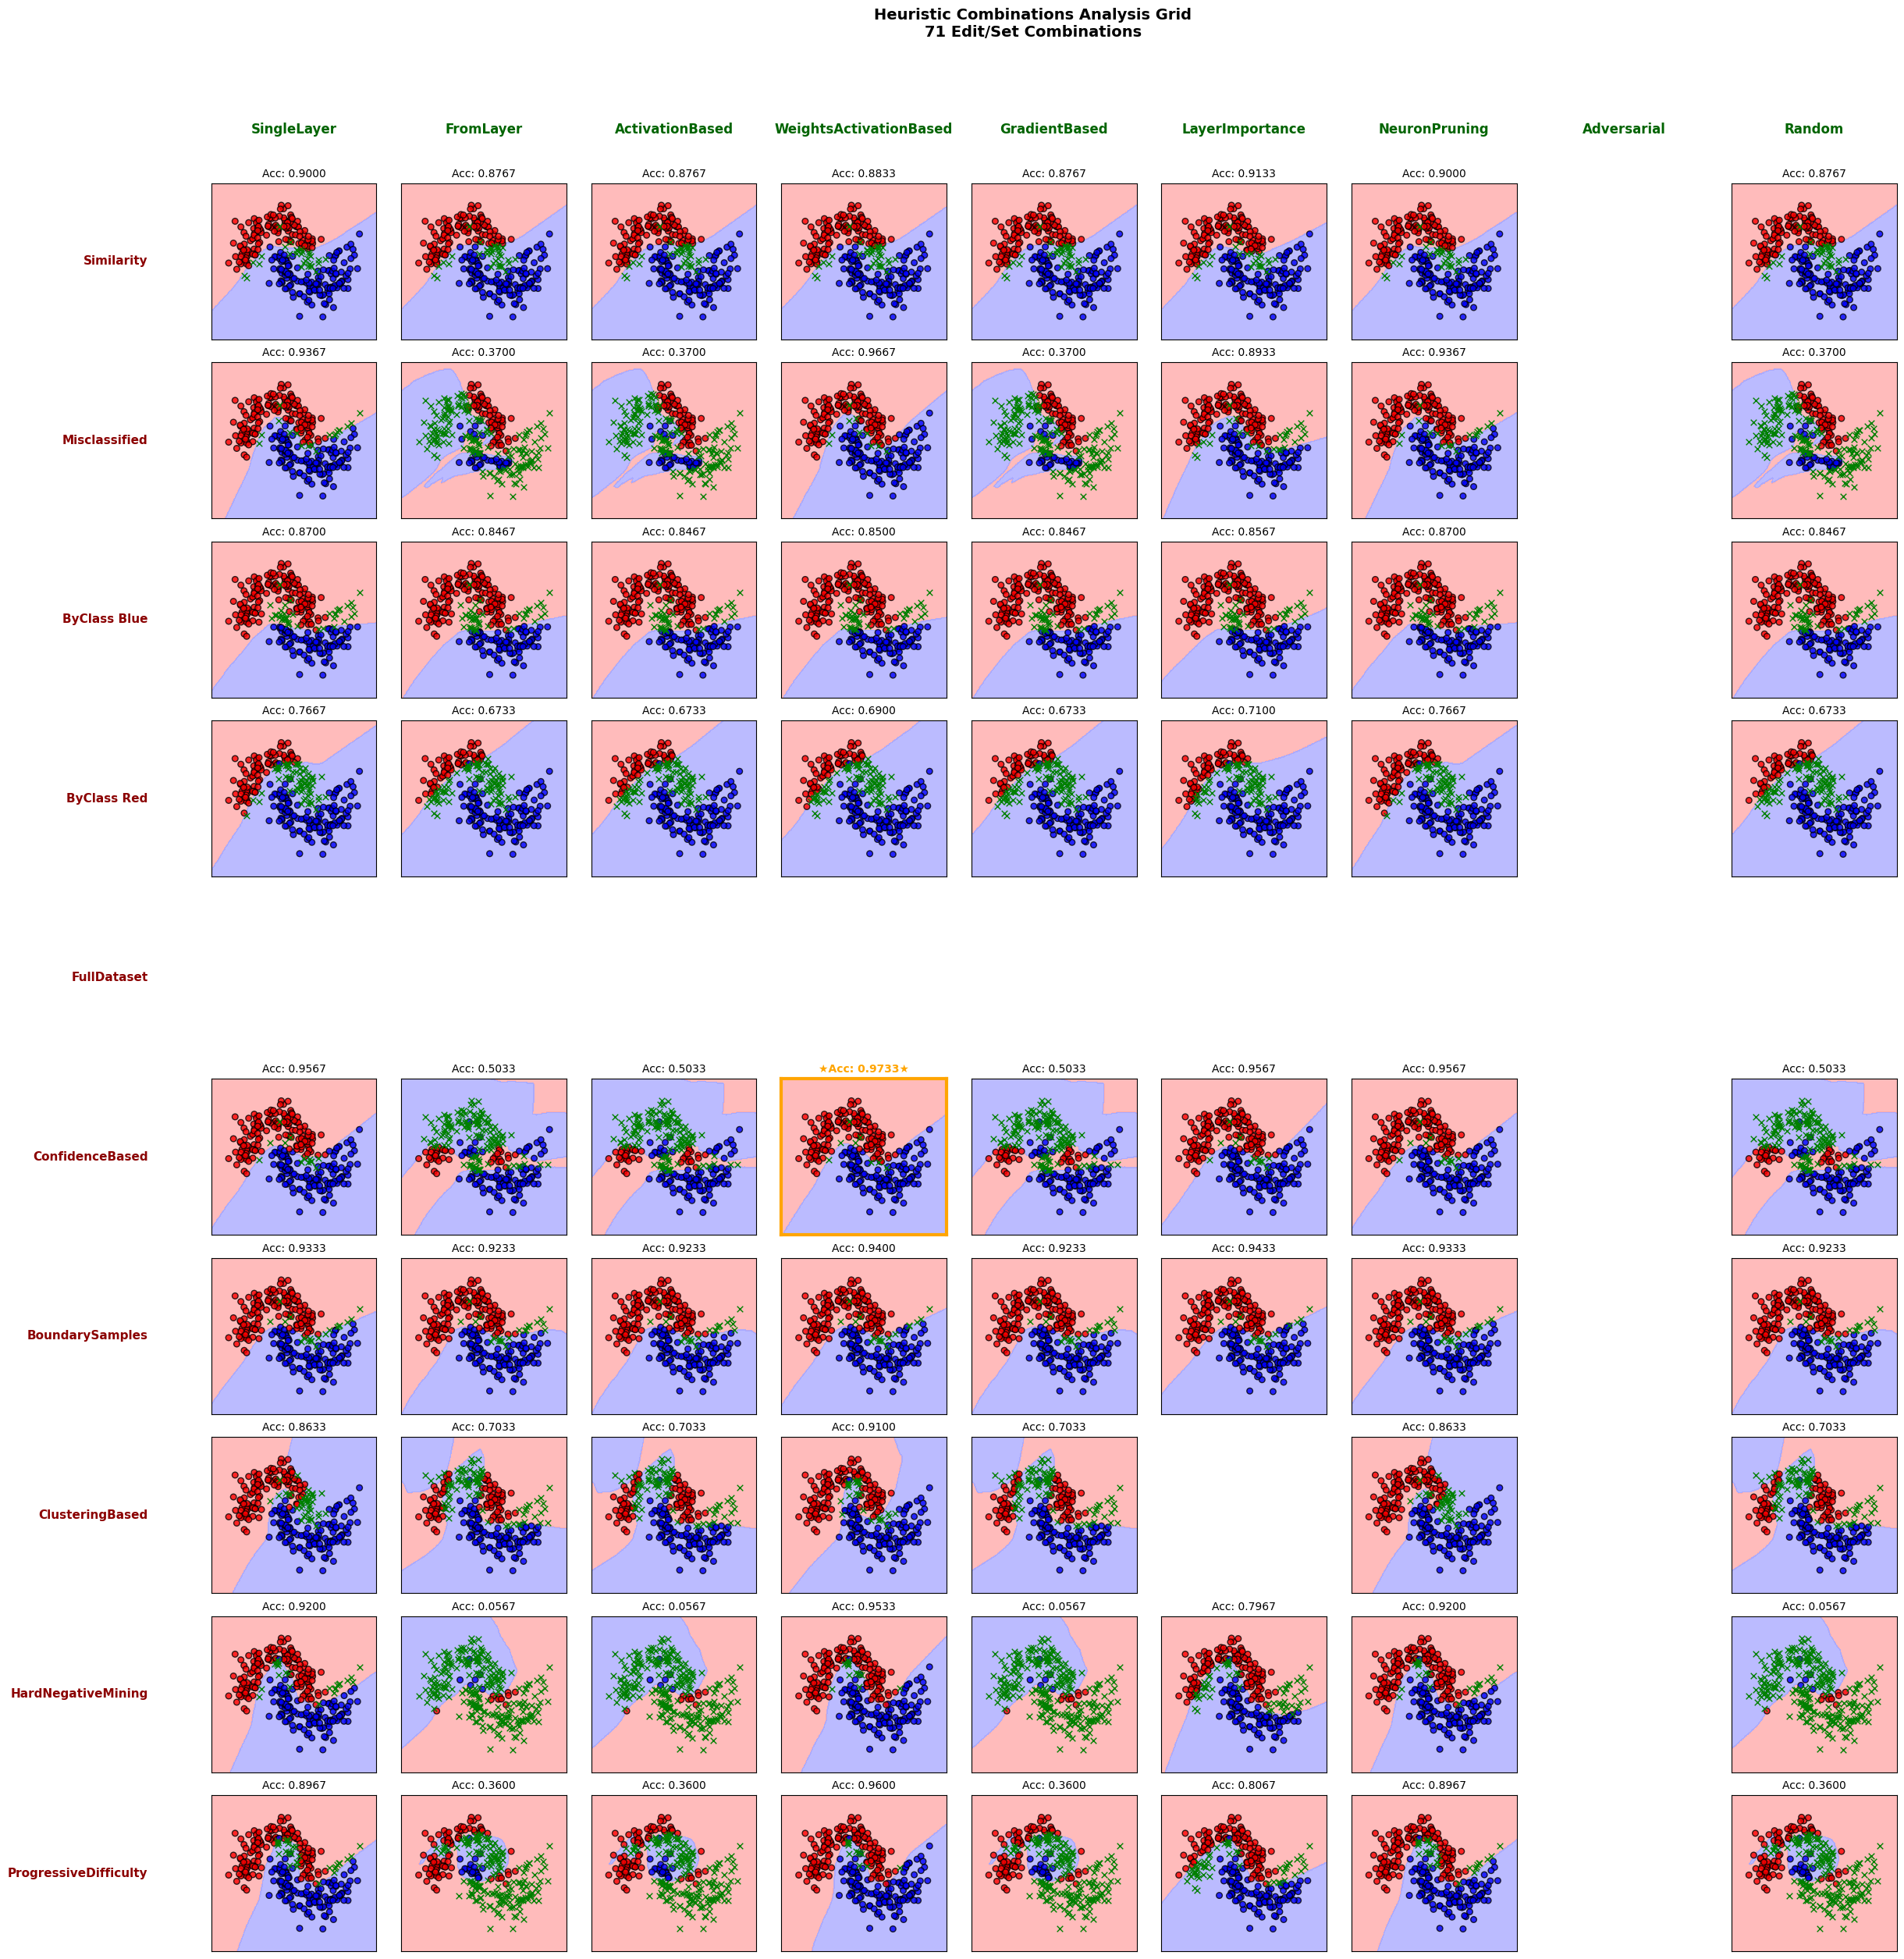
\includegraphics[width=\textwidth]{combinations.png}
	\caption{Performance visualization of all successful heuristic combinations in the MLP experiment, showing the distribution of accuracy improvements and degradations across different edit and set heuristic pairings.}
	\label{fig:mlp_combinations}
\end{figure}

The results presented visualized in Figure~\ref{fig:mlp_combinations} demonstrate clear patterns in heuristic effectiveness.
Notice the fact that the columns for Adversarial and FullDataset set heuristics are entirely empty, indicating that these combinations failed to produce valid repairs.

\subsubsection{Key Findings from MLP Experiments}

Our MLP experiments revealed several critical insights about heuristic effectiveness:

\textbf{Superior Performance of WeightsActivationBased:} The WeightsActivationBased edit heuristic emerged as the clear winner, appearing in the top-performing combination (WeightsActivationBased + ConfidenceBased) that achieved 97.33\% accuracy—a substantial +3.66\% improvement over the baseline. This heuristic consistently outperformed others across multiple set heuristics, demonstrating robust effectiveness.

\textbf{Importance of Targeted Set Selection:} The ConfidenceBased set heuristic proved highly effective, enabling the best overall performance when paired with appropriate edit heuristics. This suggests that focusing on low-confidence predictions provides a more principled approach to identifying repair targets than simple misclassification-based methods.

\textbf{Parameter Editing Intuition for Simple Models:} The success of parameter modification heuristics aligns with intuitive understanding of how simple neural networks function. For MLPs with clear decision boundaries, targeted weight adjustments can effectively shift these boundaries to correct misclassifications without significantly disrupting the overall learned representation. This is analogous to adjusting coefficients in a polynomial function to better fit data points.

\textbf{Failure Patterns and Robustness:} Several combinations failed entirely, particularly those involving the Adversarial edit heuristic (8 failures) and the FullDataset set heuristic (all 9 combinations failed). This suggests that some approaches may be fundamentally incompatible with certain repair formulations or may require different constraint parameterizations.

\textbf{Performance Distribution:} Successful repairs showed a wide range of outcomes, from significant improvements (+3.66\%) to substantial degradations (-88.0\%). This variability underscores the importance of principled heuristic selection rather than arbitrary choices.

\subsection{CNN Analysis on Image Classification}

We conducted complementary experiments on AlexNet trained on CIFAR-10 to understand how heuristic effectiveness scales to more complex architectures and higher-dimensional problems.

\subsubsection{Deterministic vs. Stochastic Repair Strategies}

\begin{description}
	\item[Deterministic ("full-set") repair] in which we solve a single repair problem over an entire edit set of varying size and homogeneity.
	\item[Stochastic ("incremental") repair] in which we perform repeated, small-batch repair passes—carrying forward the model between passes—so as to trade batch size, number of passes, and homogeneity against overall fidelity.
\end{description}

Our CNN experiments used a pretrained AlexNet model with baseline test accuracy of 72.08\% on CIFAR-10, allowing us to measure how each strategy trades off global test accuracy against local repair accuracy.

\subsubsection{Repair Set Size Impact}

Our experiments demonstrate that larger repair sets consistently lead to worse performance across all metrics. As repair set size increases from 10 to 200 examples, we observe dramatic degradation in success rates, increased accuracy drawdown, and longer repair times.

\begin{figure}[h]
	\centering
	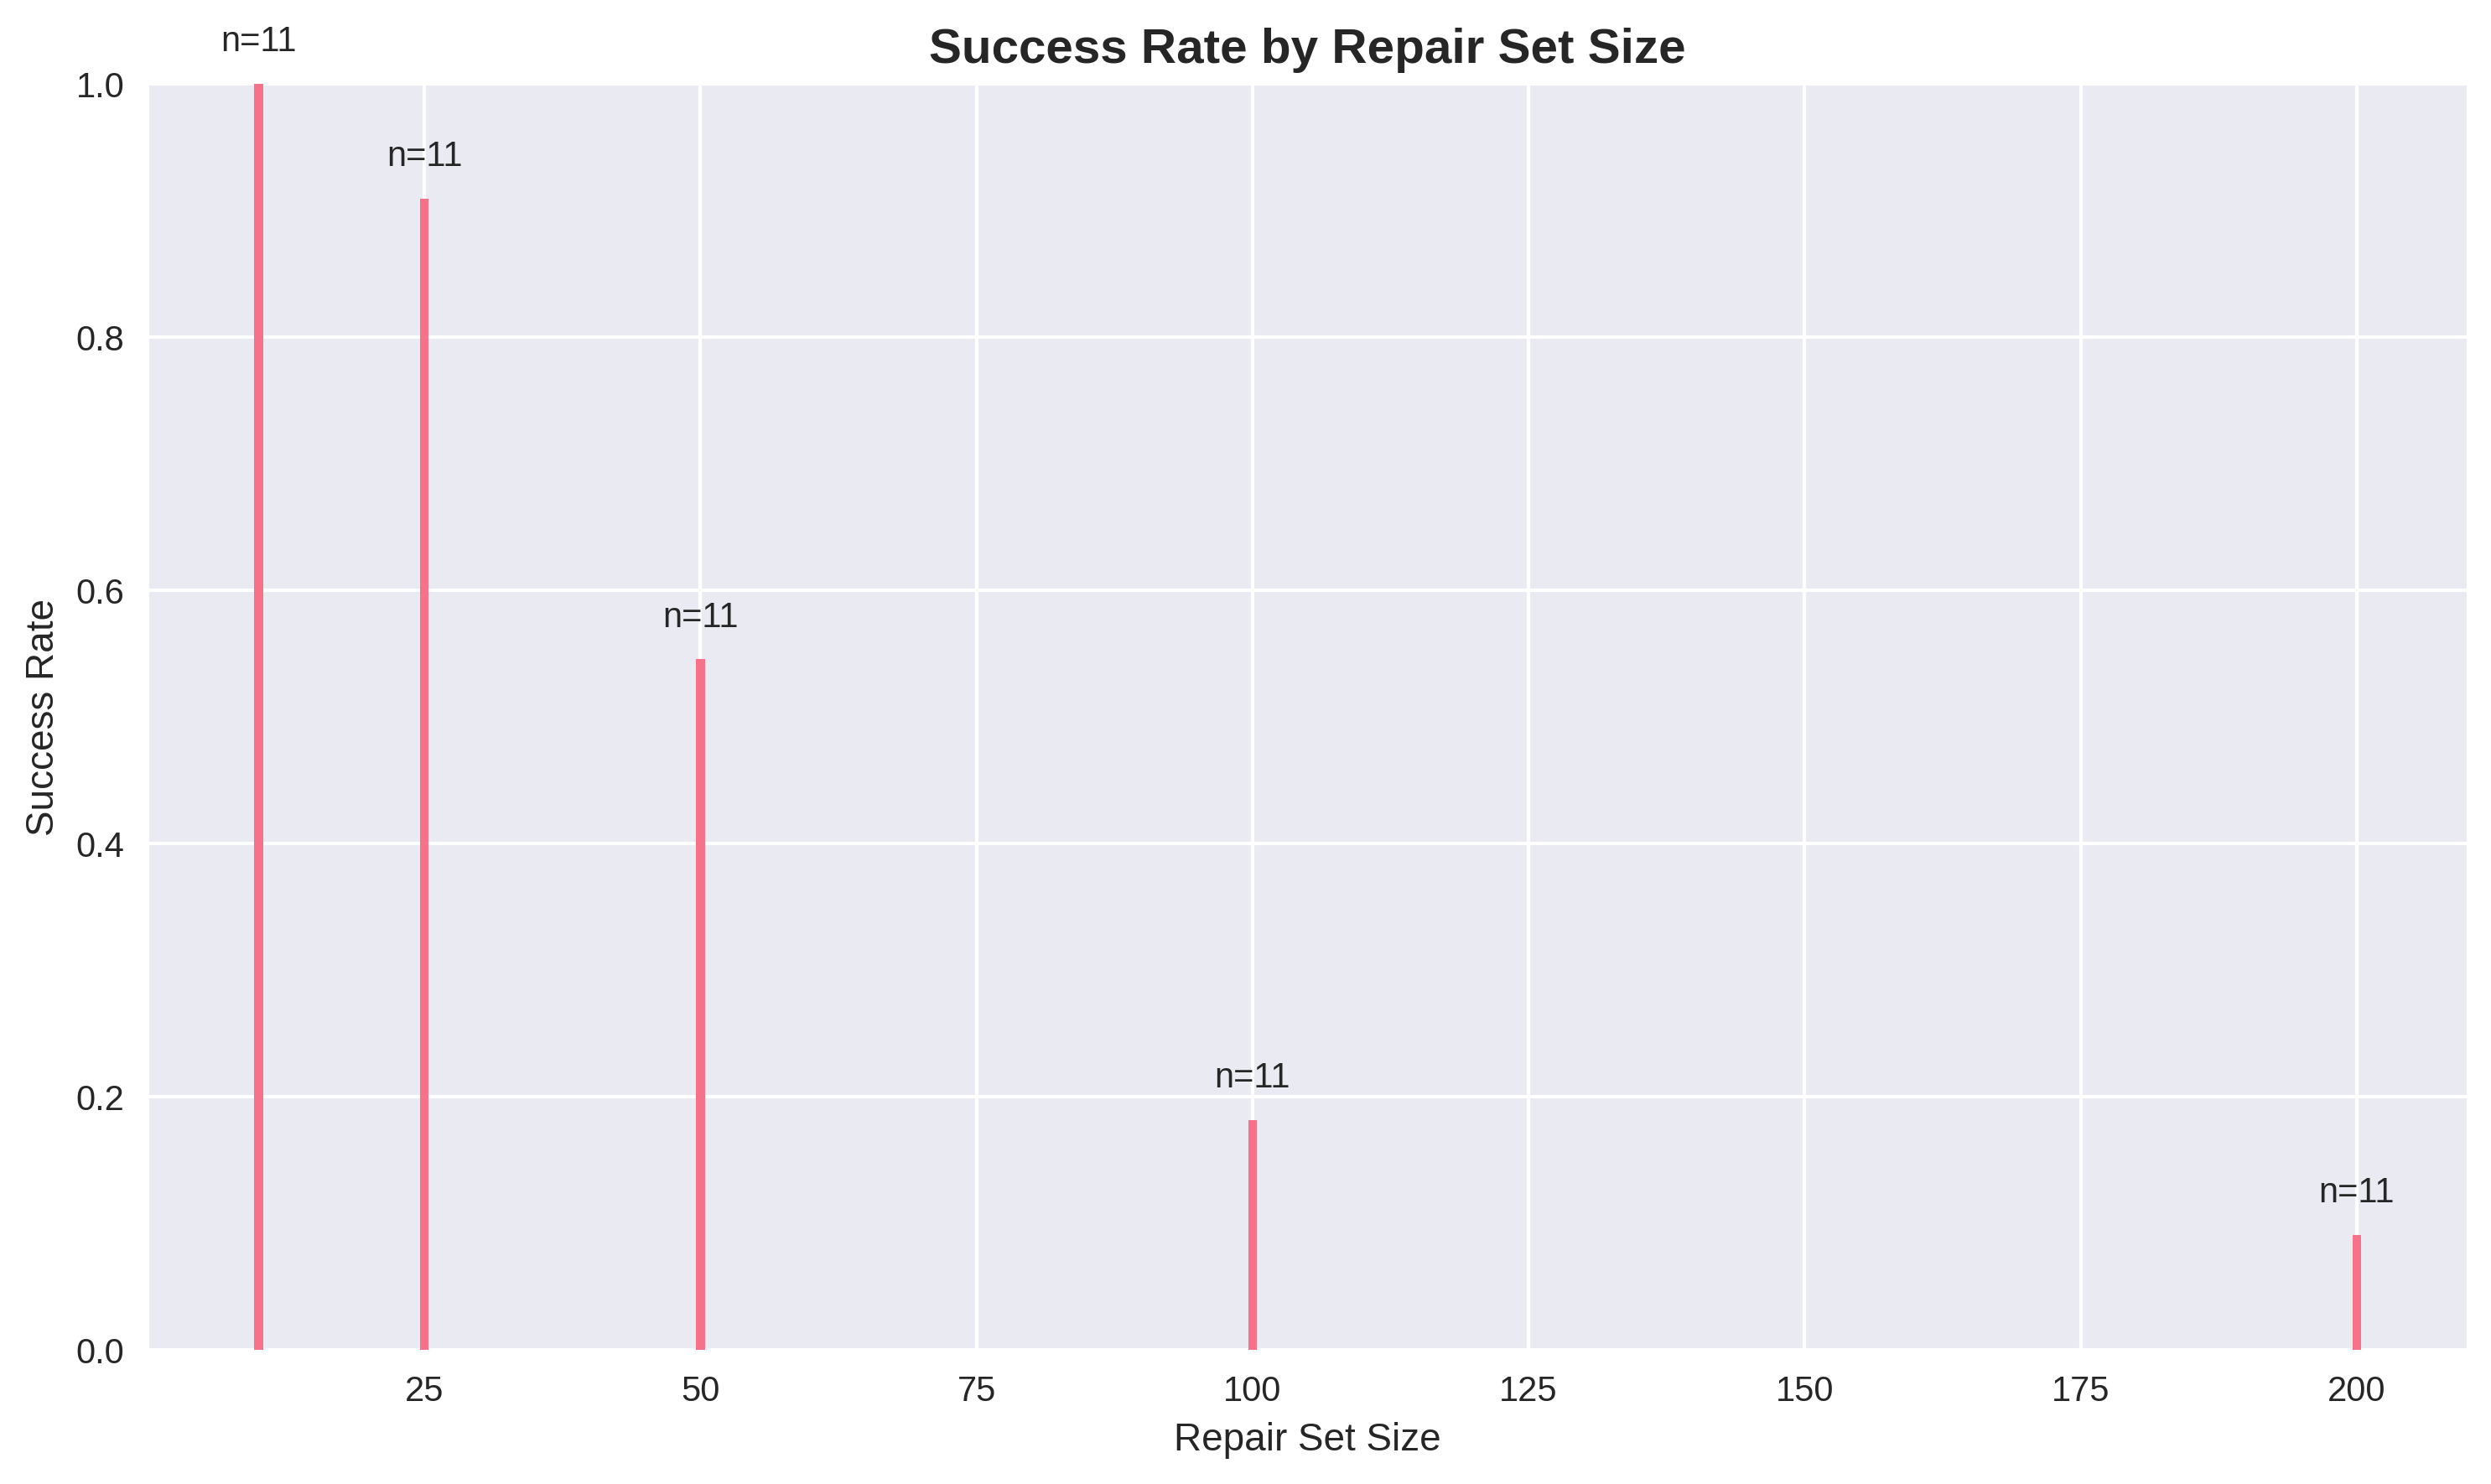
\includegraphics[width=0.8\textwidth]{results/one_shot_analysis/success_rates/success_rate_by_size.png}
	\caption{Success rate by repair set size, showing dramatic degradation in repair feasibility as set size increases beyond 25 examples.}
	\label{fig:success_rate_by_size}
\end{figure}

\begin{figure}[h]
	\centering
	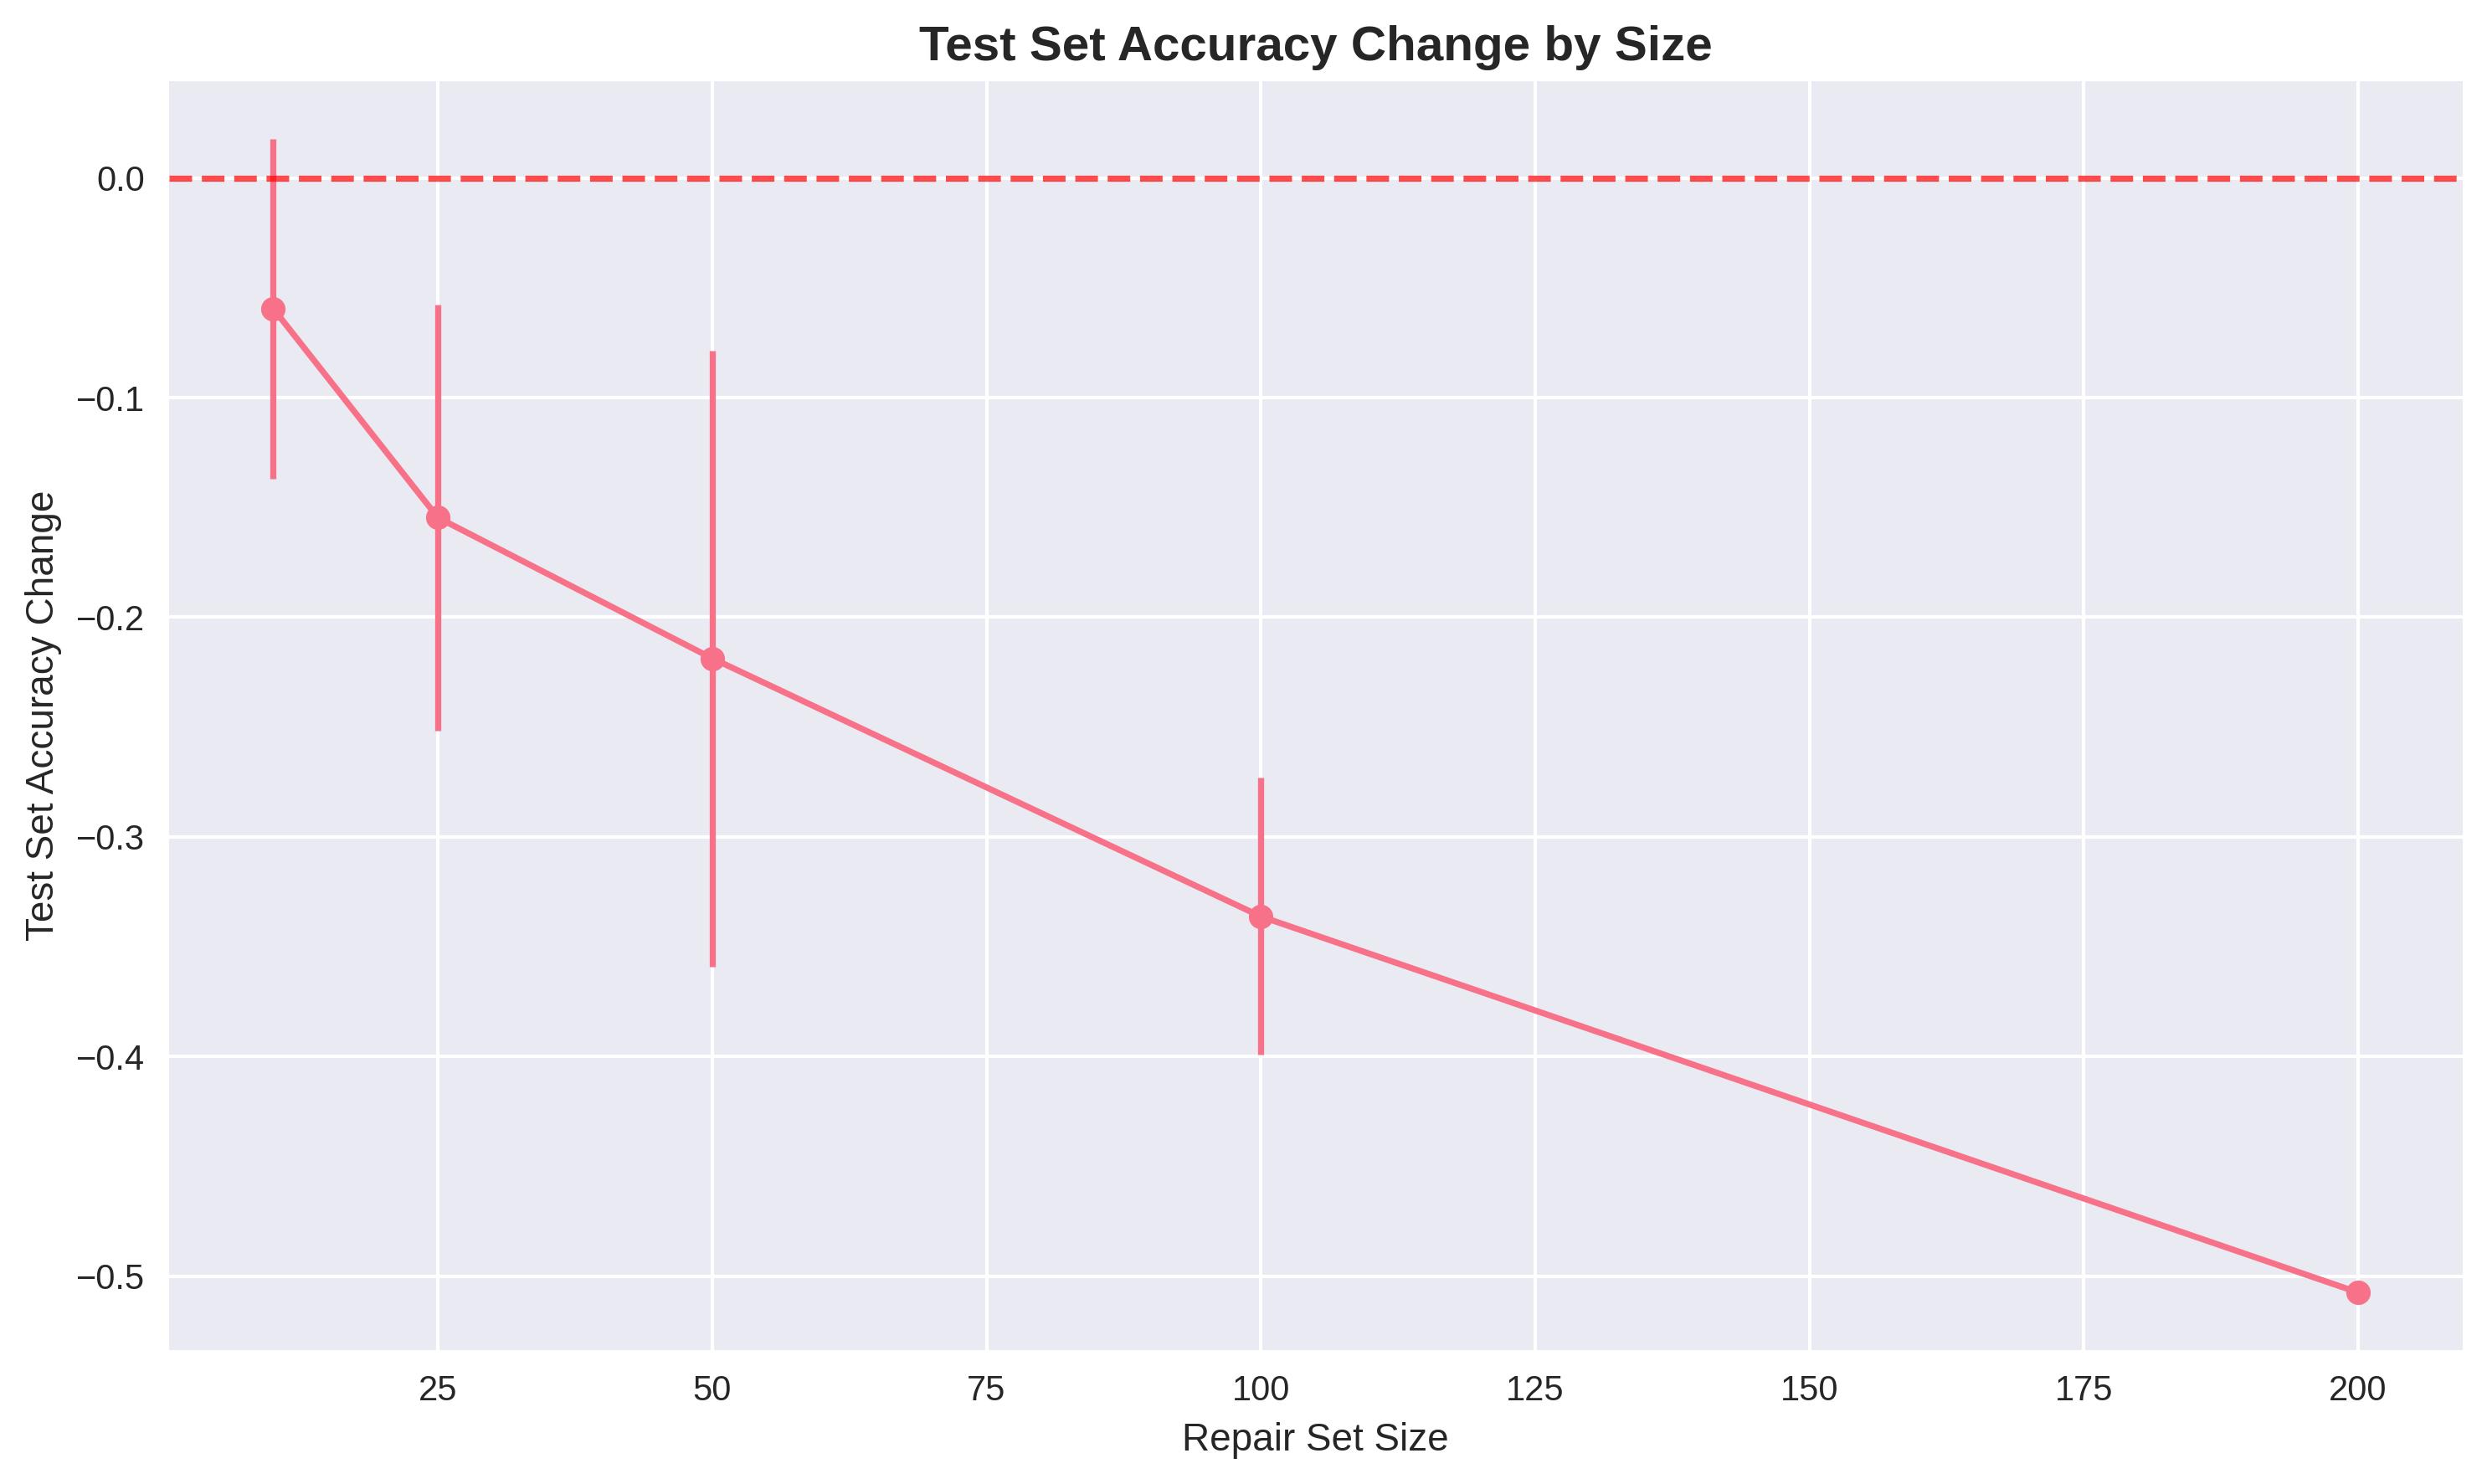
\includegraphics[width=0.8\textwidth]{results/one_shot_analysis/accuracy/accuracy_change_by_size.png}
	\caption{Test set accuracy drawdown by repair set size, demonstrating the severe trade-off between local repair success and global model performance as repair set size increases.}
	\label{fig:accuracy_drawdown_by_size}
\end{figure}

The data shows clear trends across all metrics:
\begin{itemize}
	\item \textbf{Success Rate:} Drops from 100\% for size 10 to just 9.1\% for size 200
	\item \textbf{Accuracy Drawdown:} Increases from minimal impact (~-2.7\%) for small sets to severe degradation (-50.8\%) for large sets
	\item \textbf{Repair Time:} Scales linearly from ~10 seconds to ~50 seconds as set size increases
\end{itemize}

\subsubsection{Repair Set Homogeneity Effects}

Repair set composition significantly impacts both success rates and performance degradation patterns. Class-homogeneous sets consistently outperform misclassified sets across all metrics.

\begin{figure}[h]
	\centering
	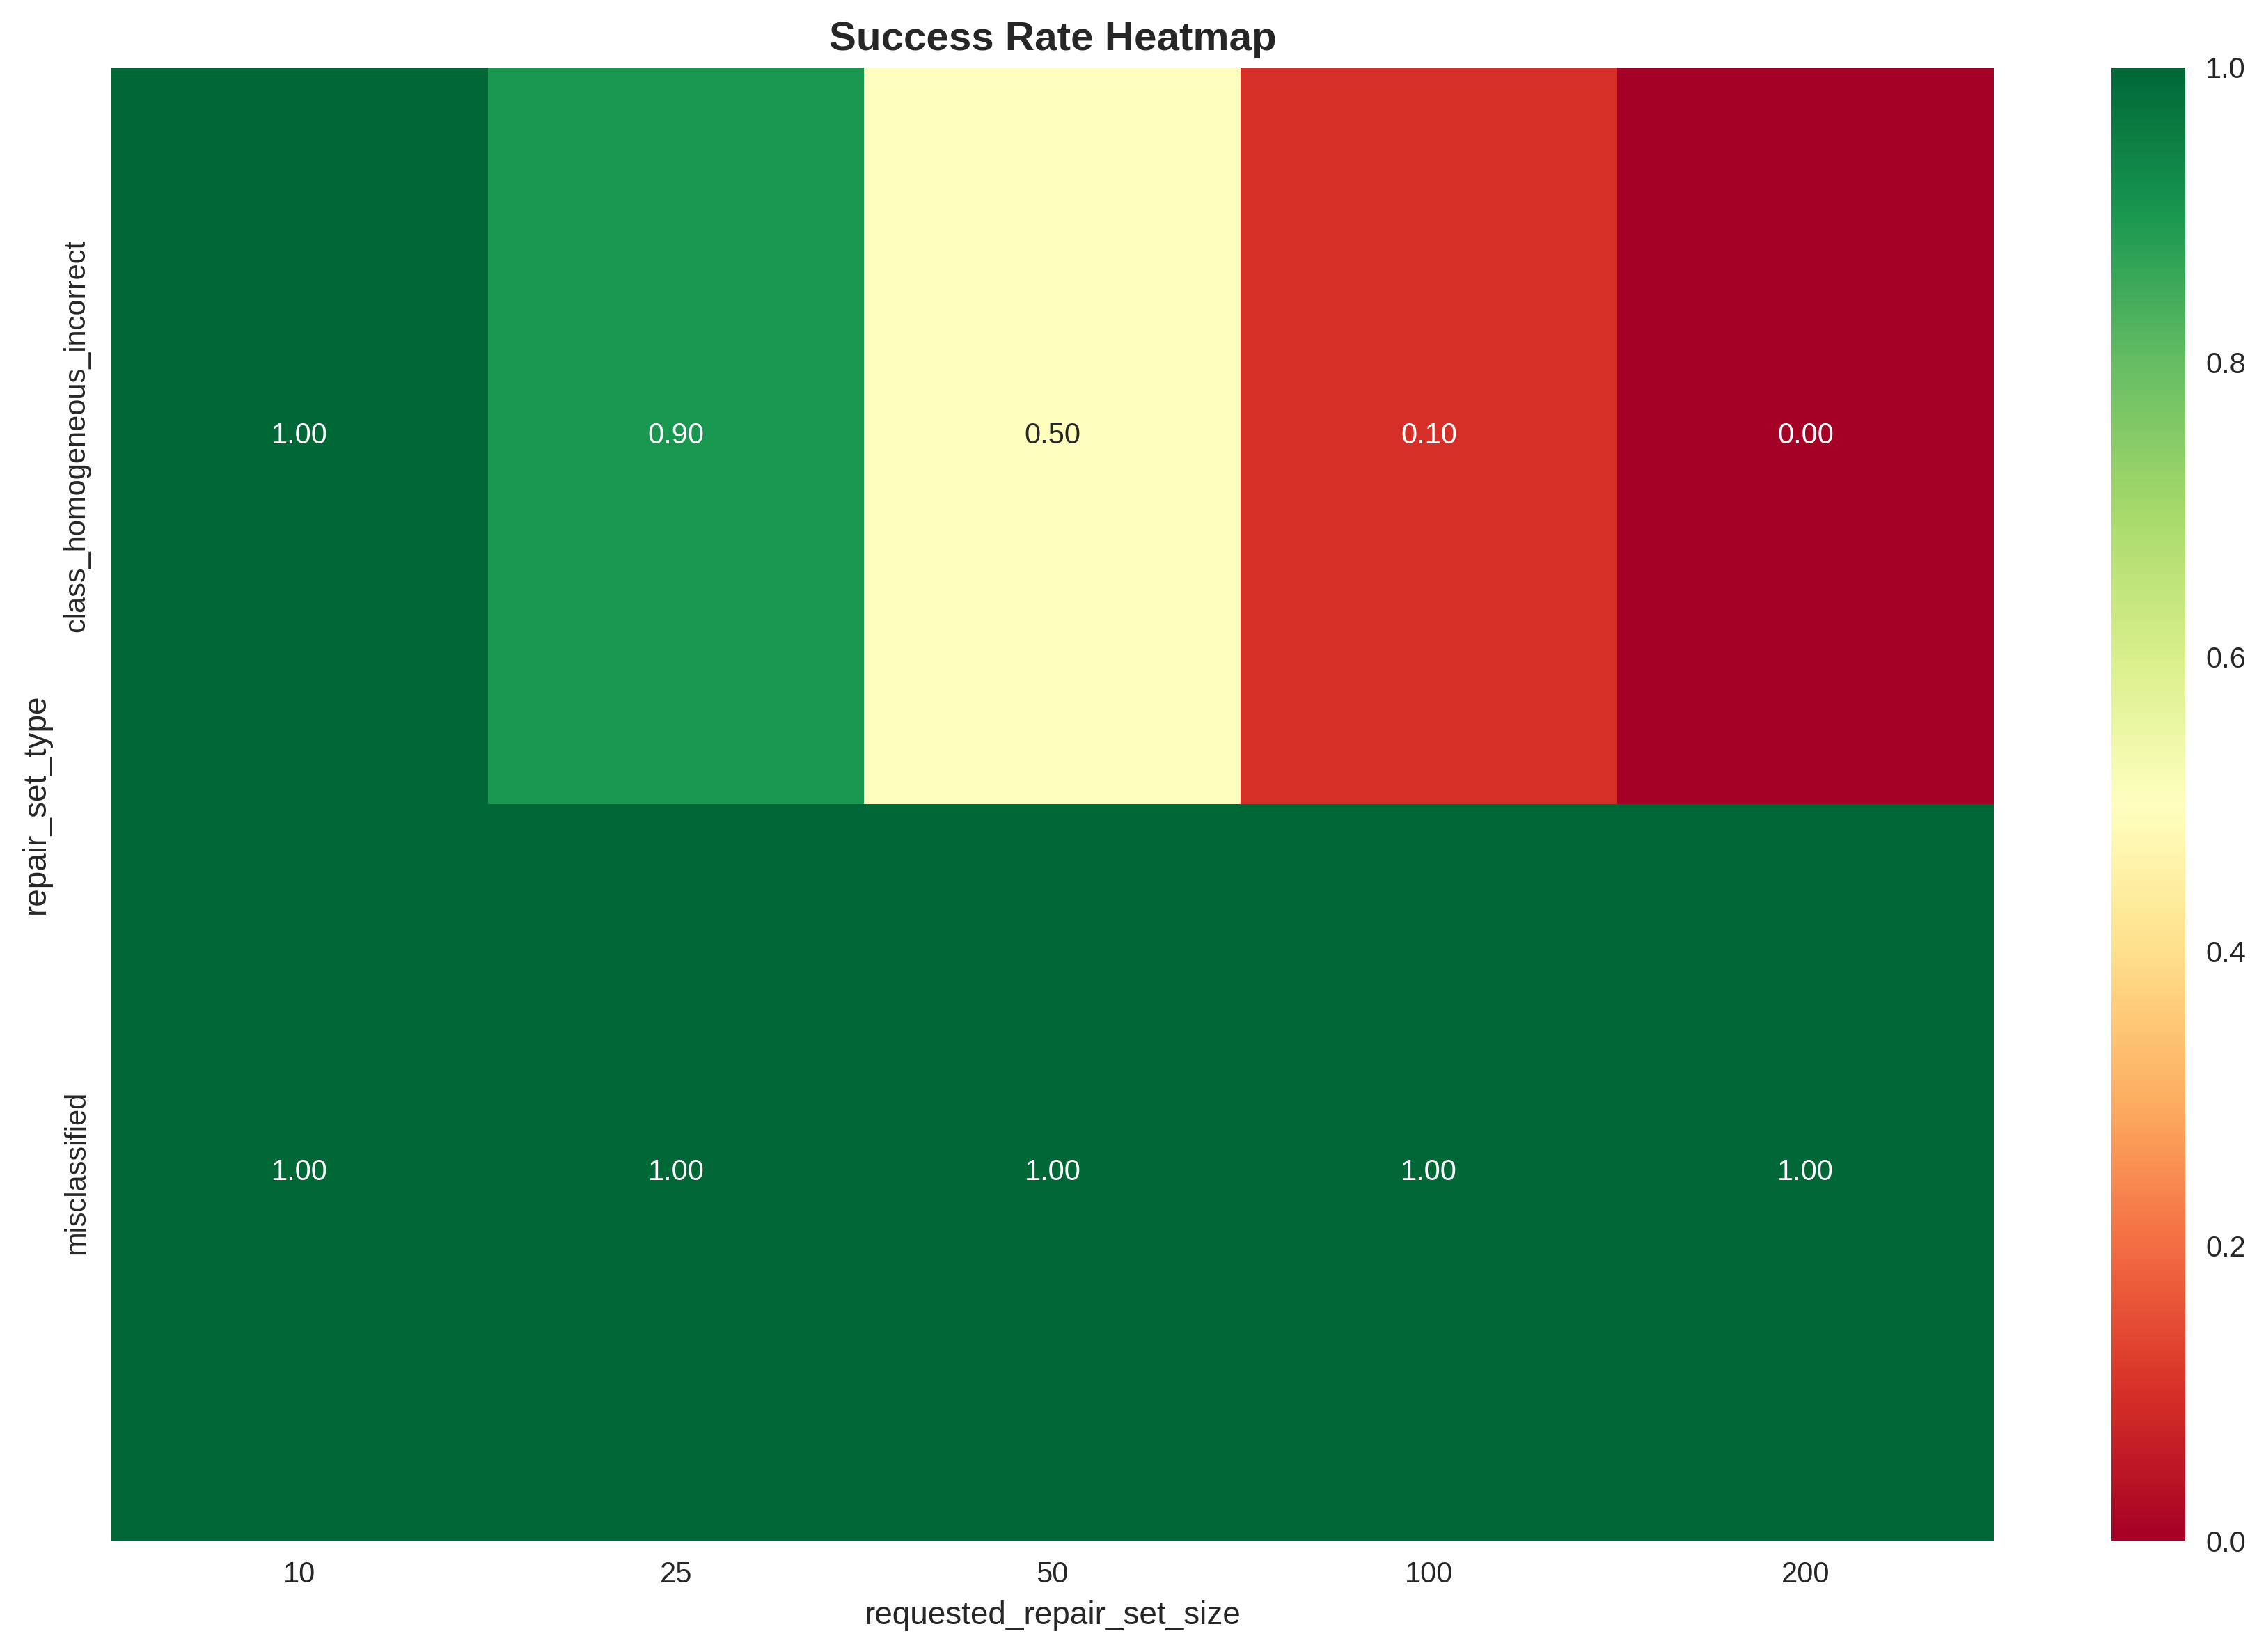
\includegraphics[width=0.8\textwidth]{results/one_shot_analysis/success_rates/success_rate_heatmap.png}
	\caption{Success rate heatmap showing the interaction between repair set type and size, clearly illustrating the feasibility boundaries for different repair strategies.}
	\label{fig:success_rate_heatmap}
\end{figure}

\begin{figure}[h]
	\centering
	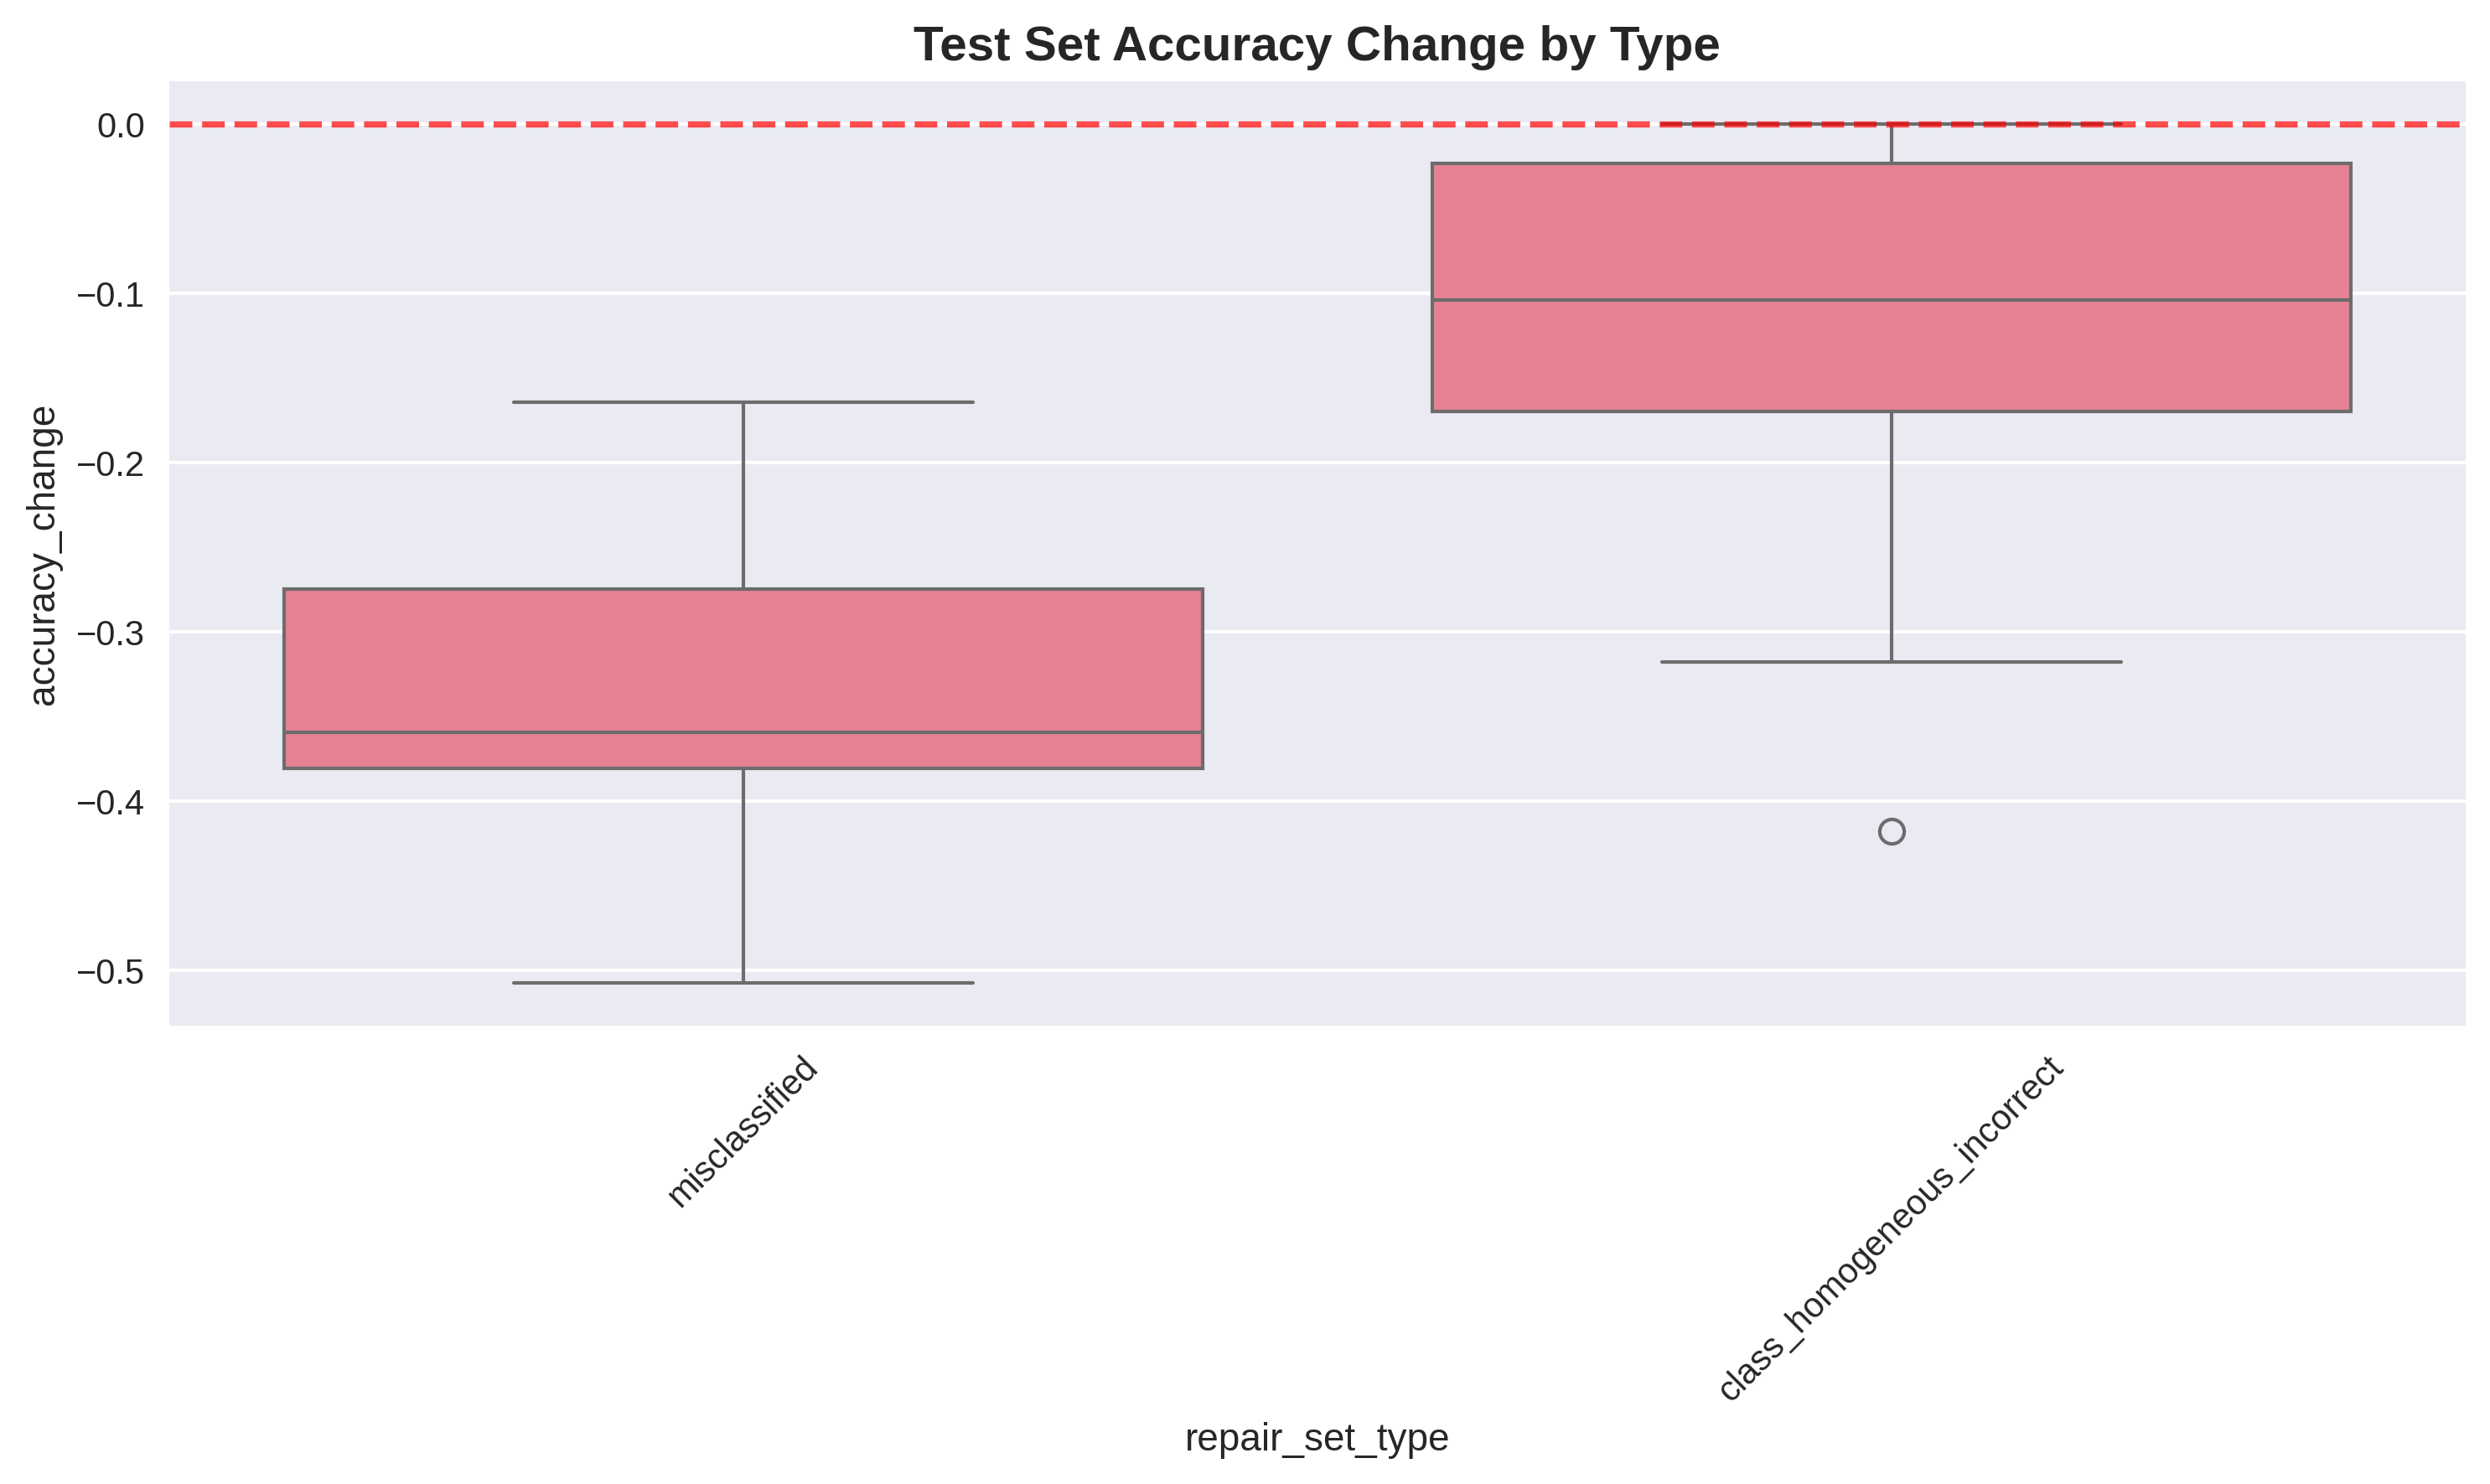
\includegraphics[width=0.8\textwidth]{results/one_shot_analysis/accuracy/accuracy_change_by_type.png}
	\caption{Accuracy drawdown distribution by repair set type, demonstrating that class-homogeneous repairs cause significantly less performance degradation than misclassified repairs.}
	\label{fig:accuracy_change_by_type}
\end{figure}

\subsubsection{Stochastic Repair Efficiency for Class-Homogeneous Sets}

Our stochastic experiments focused on batch sizes of 5 and 10, as batch size 20 resulted in too many infeasible repairs. For class-homogeneous sets, stochastic repair proves highly efficient, achieving rapid convergence to near-perfect repair set accuracy.

\begin{figure}[h]
	\centering
	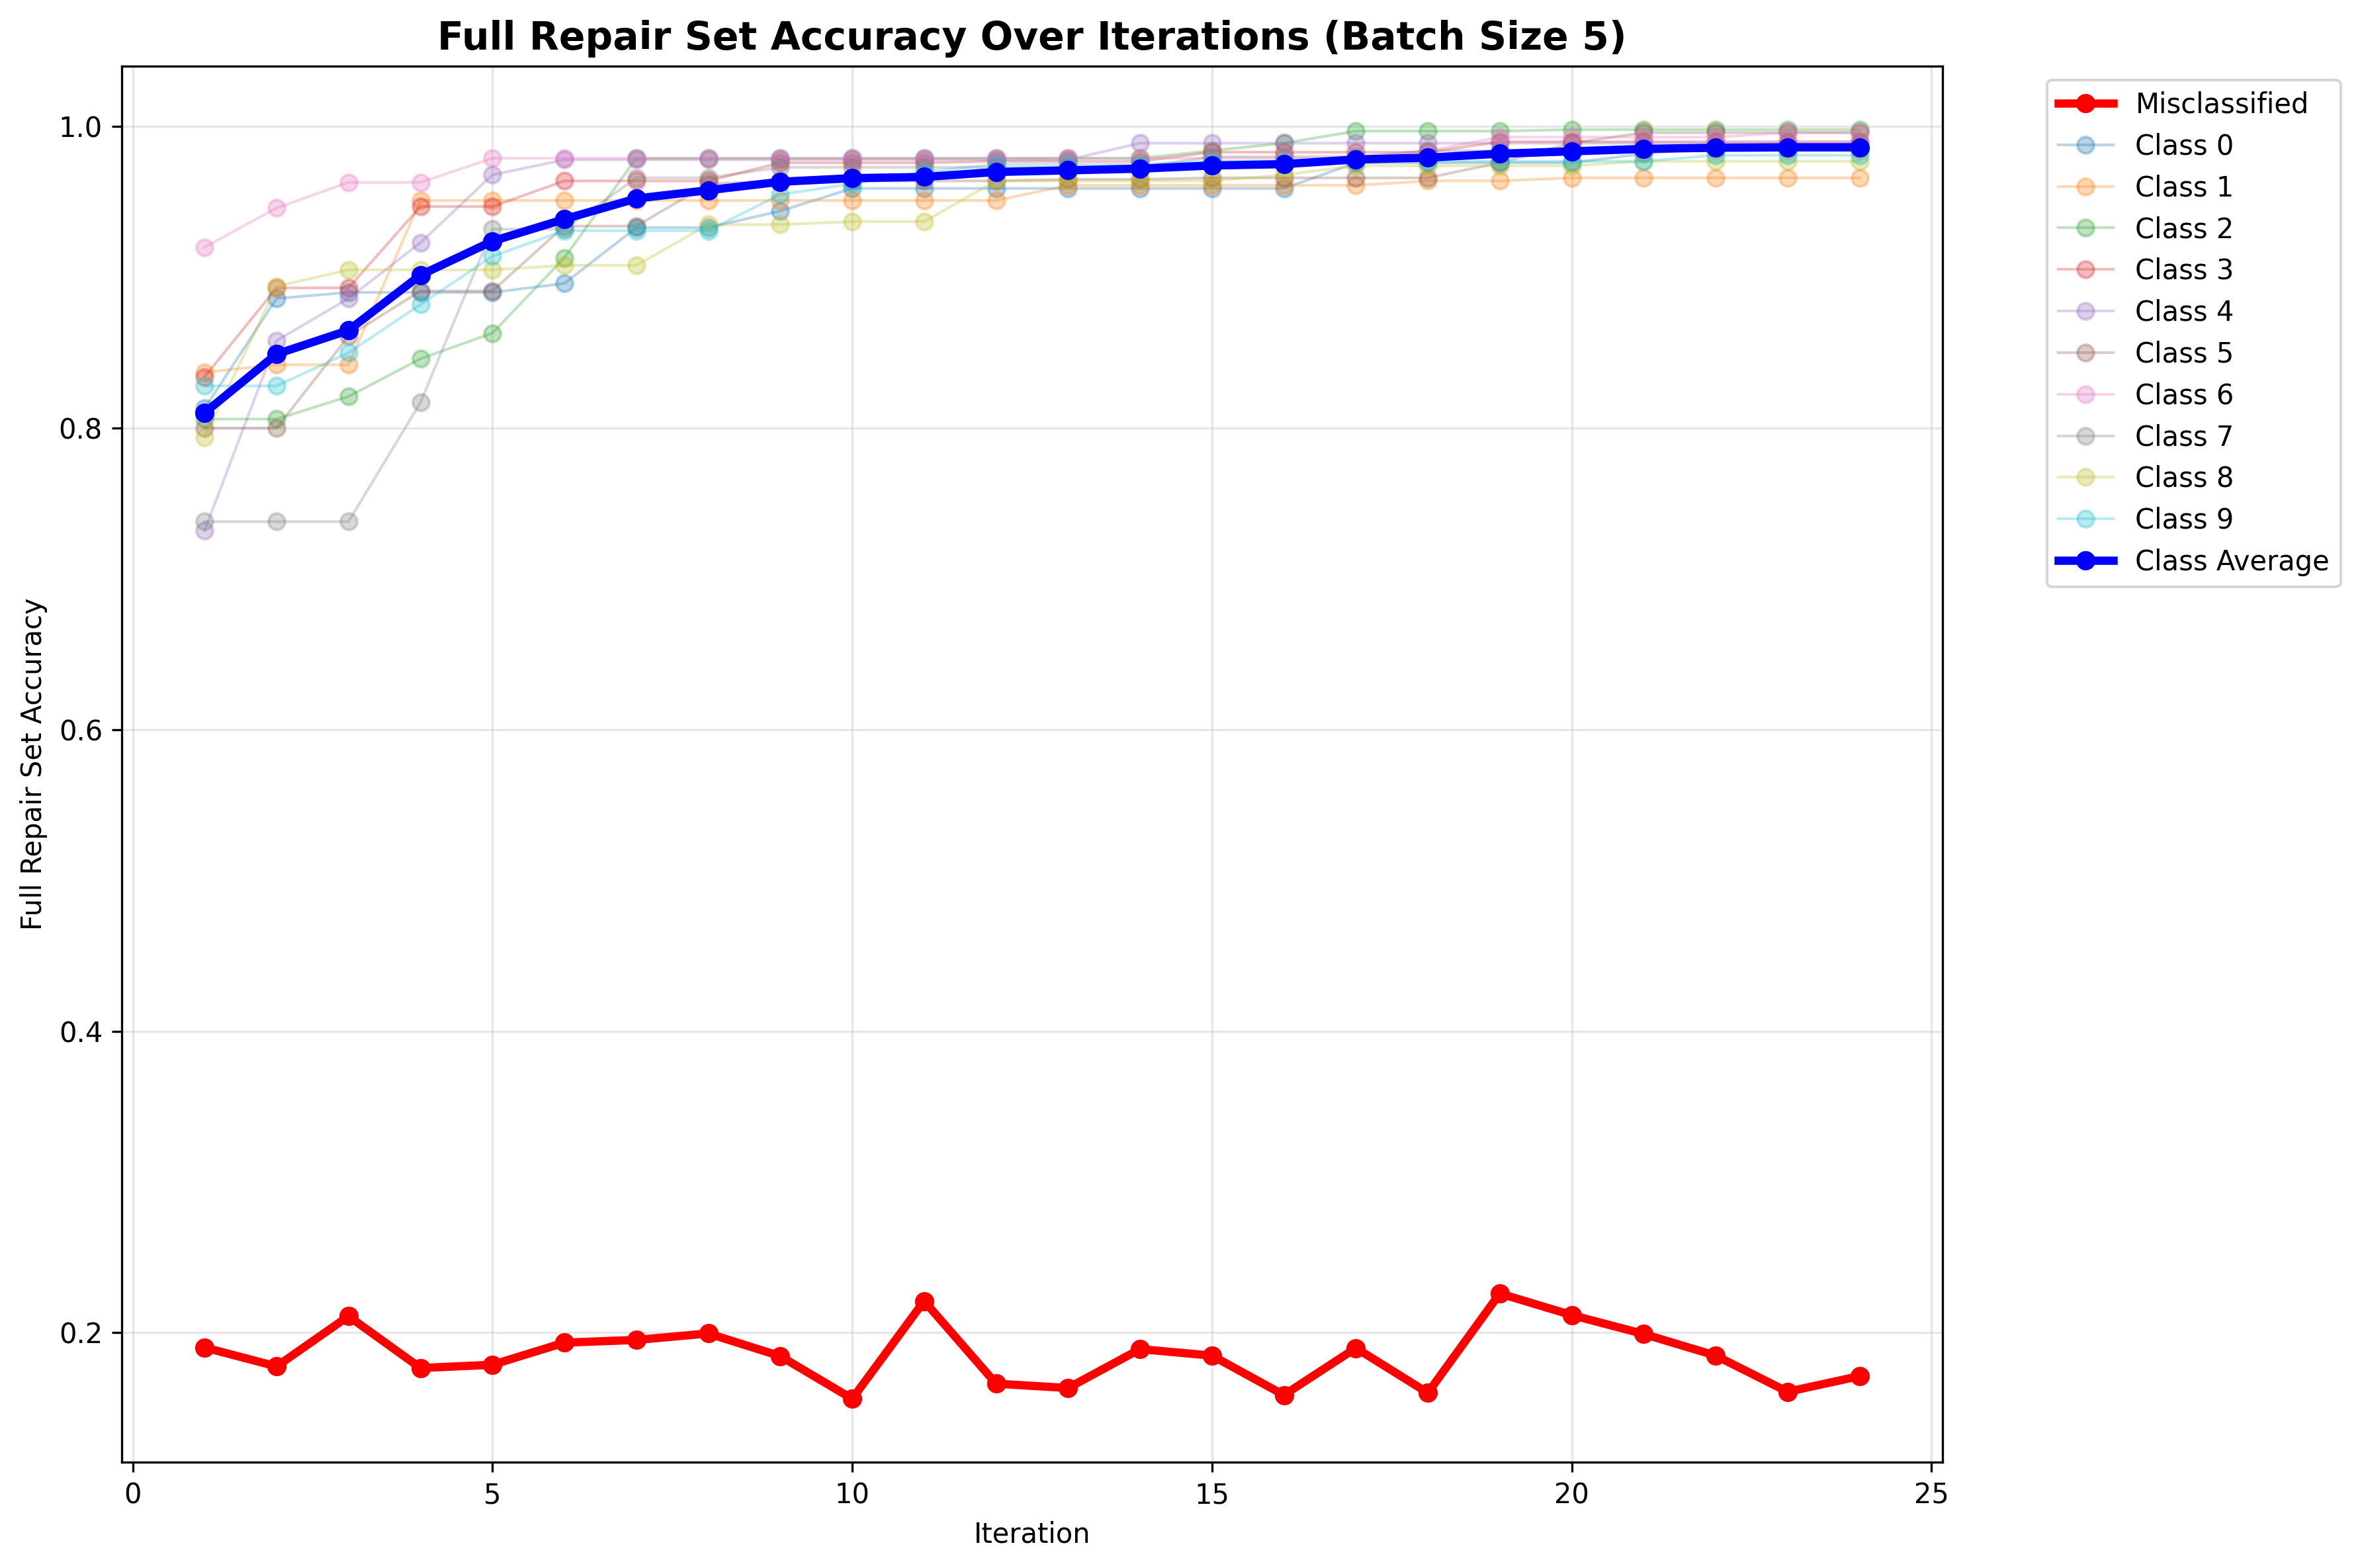
\includegraphics[width=\textwidth]{results/stochastic_analysis/batch_iterations/repair_accuracy_batch_5.png}
	\caption{Repair set accuracy evolution for batch size 5, showing rapid convergence to near-perfect accuracy within 5 iterations for class-homogeneous repairs.}
	\label{fig:repair_convergence_batch_5}
\end{figure}

\begin{figure}[h]
	\centering
	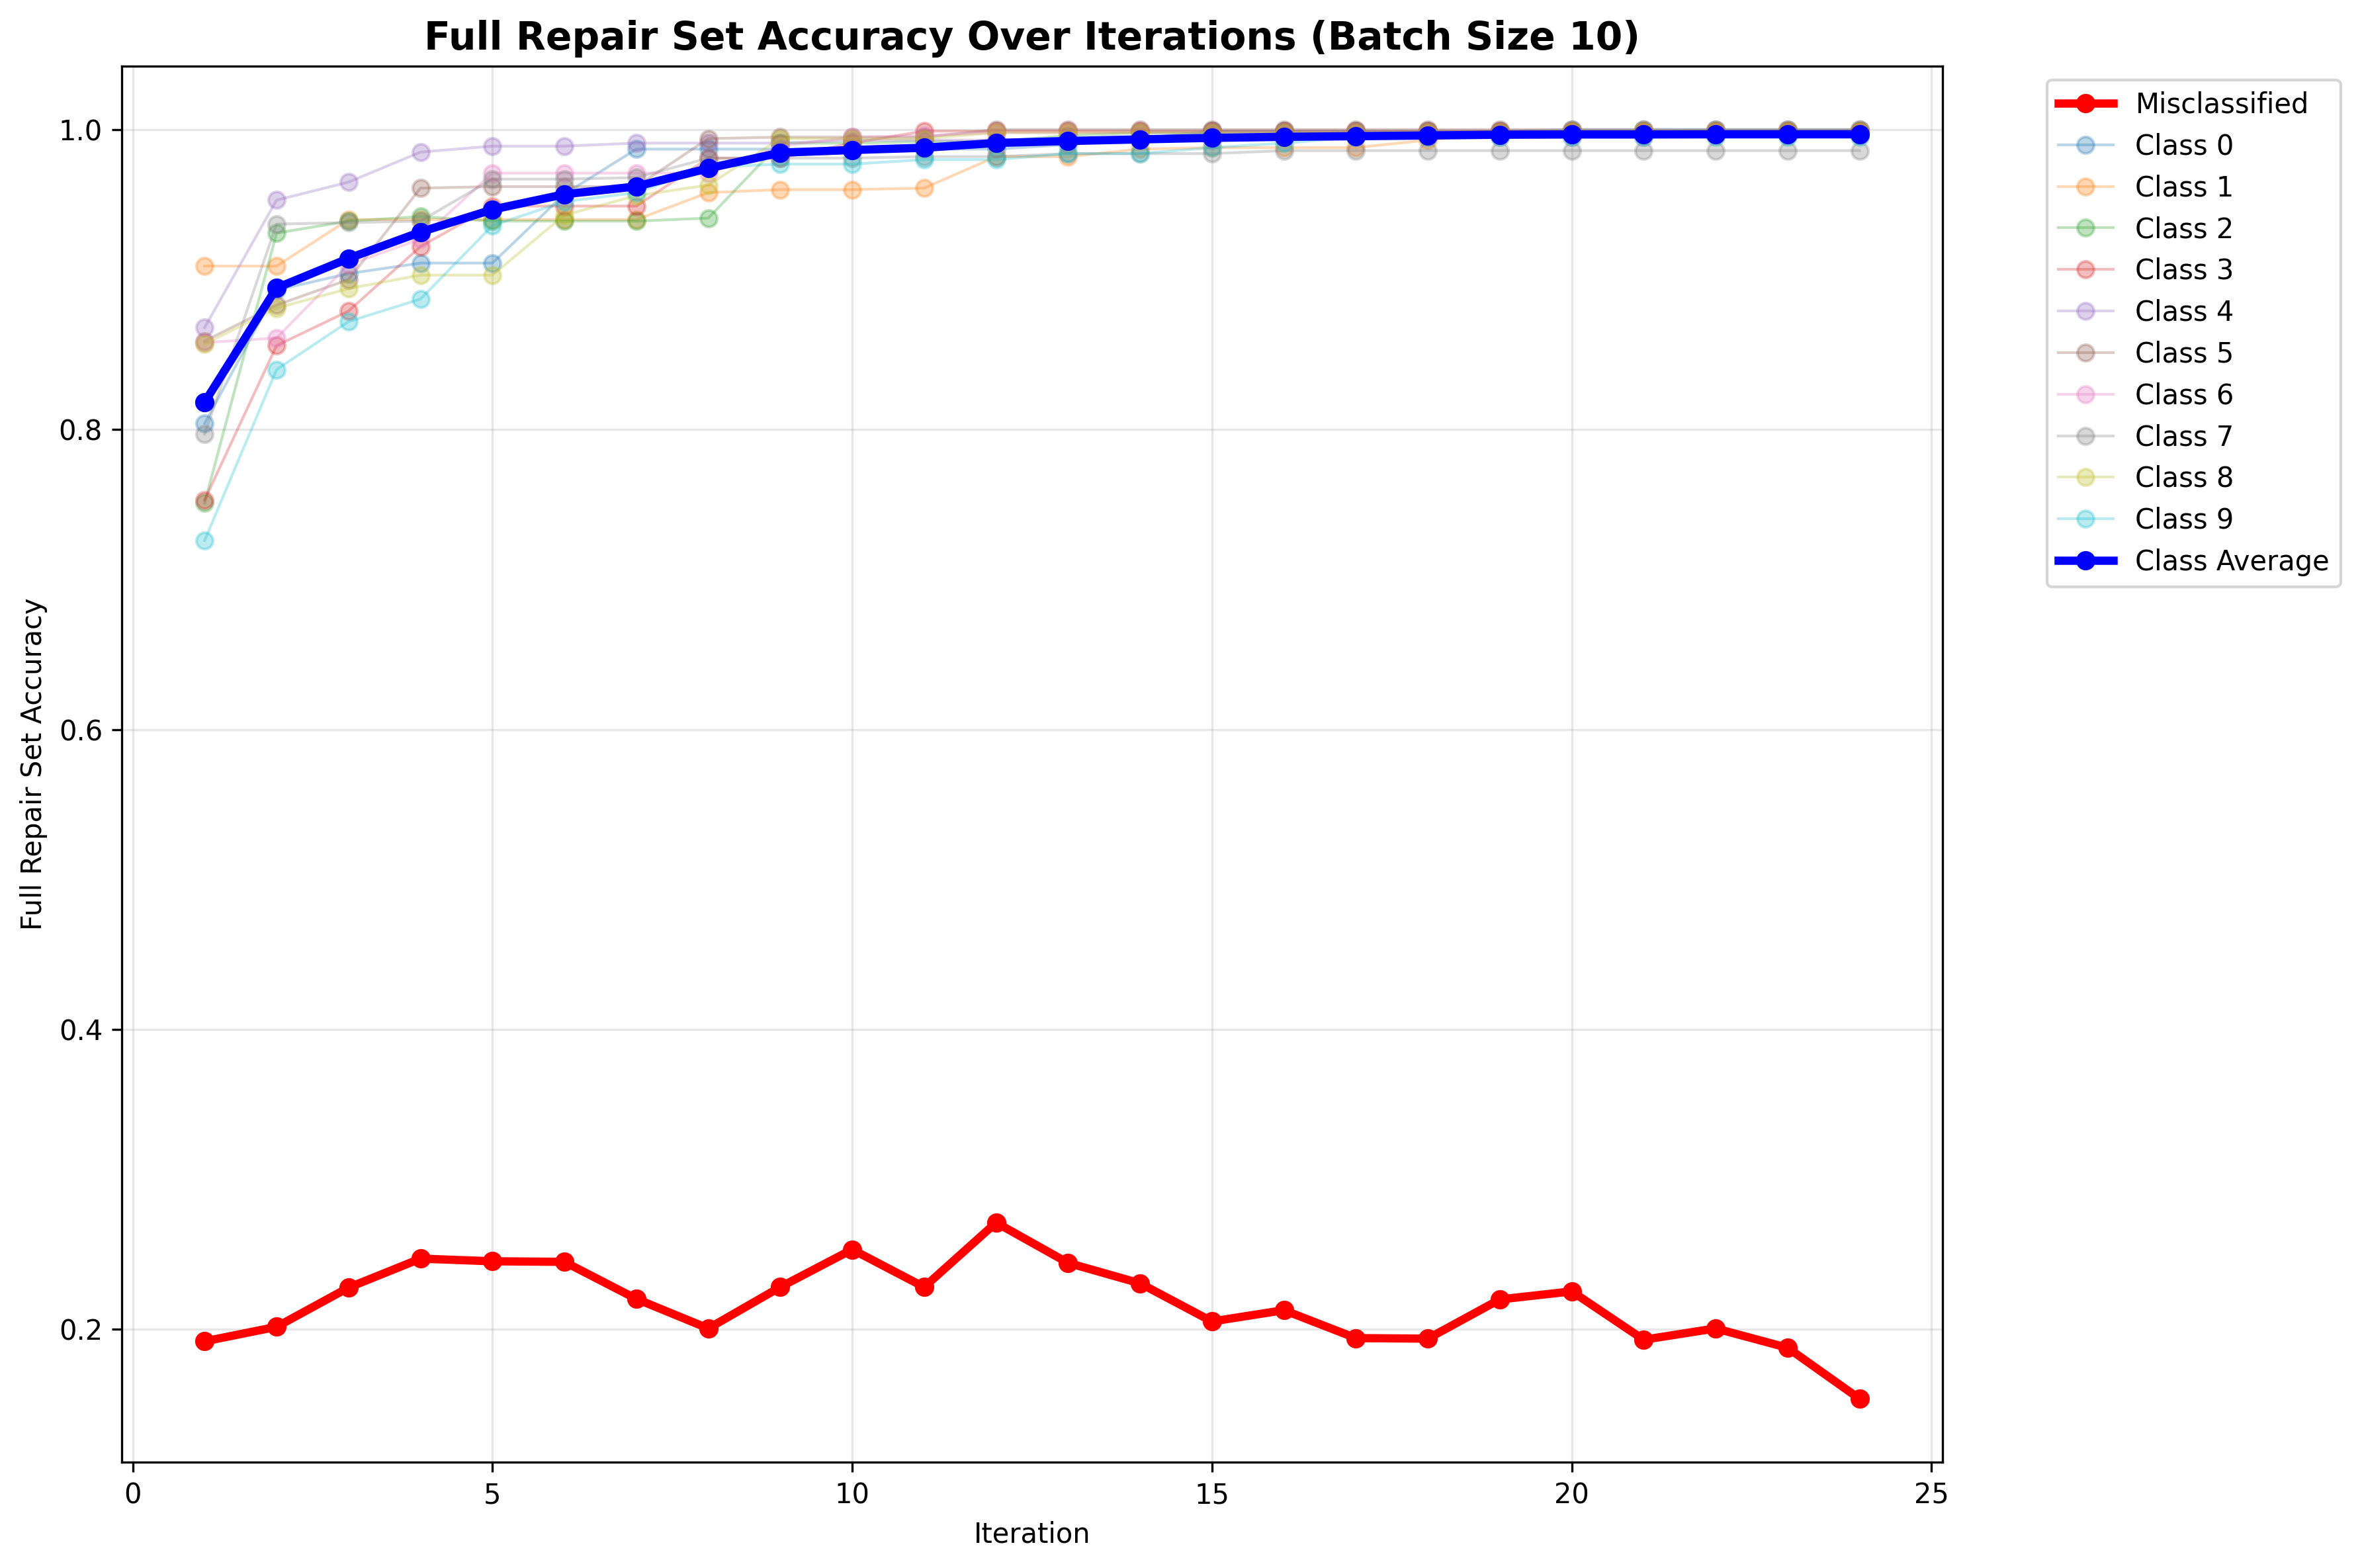
\includegraphics[width=\textwidth]{results/stochastic_analysis/batch_iterations/repair_accuracy_batch_10.png}
	\caption{Repair set accuracy evolution for batch size 10, demonstrating similar rapid convergence patterns to batch size 5.}
	\label{fig:repair_convergence_batch_10}
\end{figure}

\subsubsection{Early Stopping to Reduce Drawdown}

The key insight is that stochastic repair converges to near-perfect repair set accuracy within approximately 5 iterations. Stopping early can significantly reduce global accuracy drawdown while maintaining excellent local repair performance.

\begin{figure}[h]
	\centering
	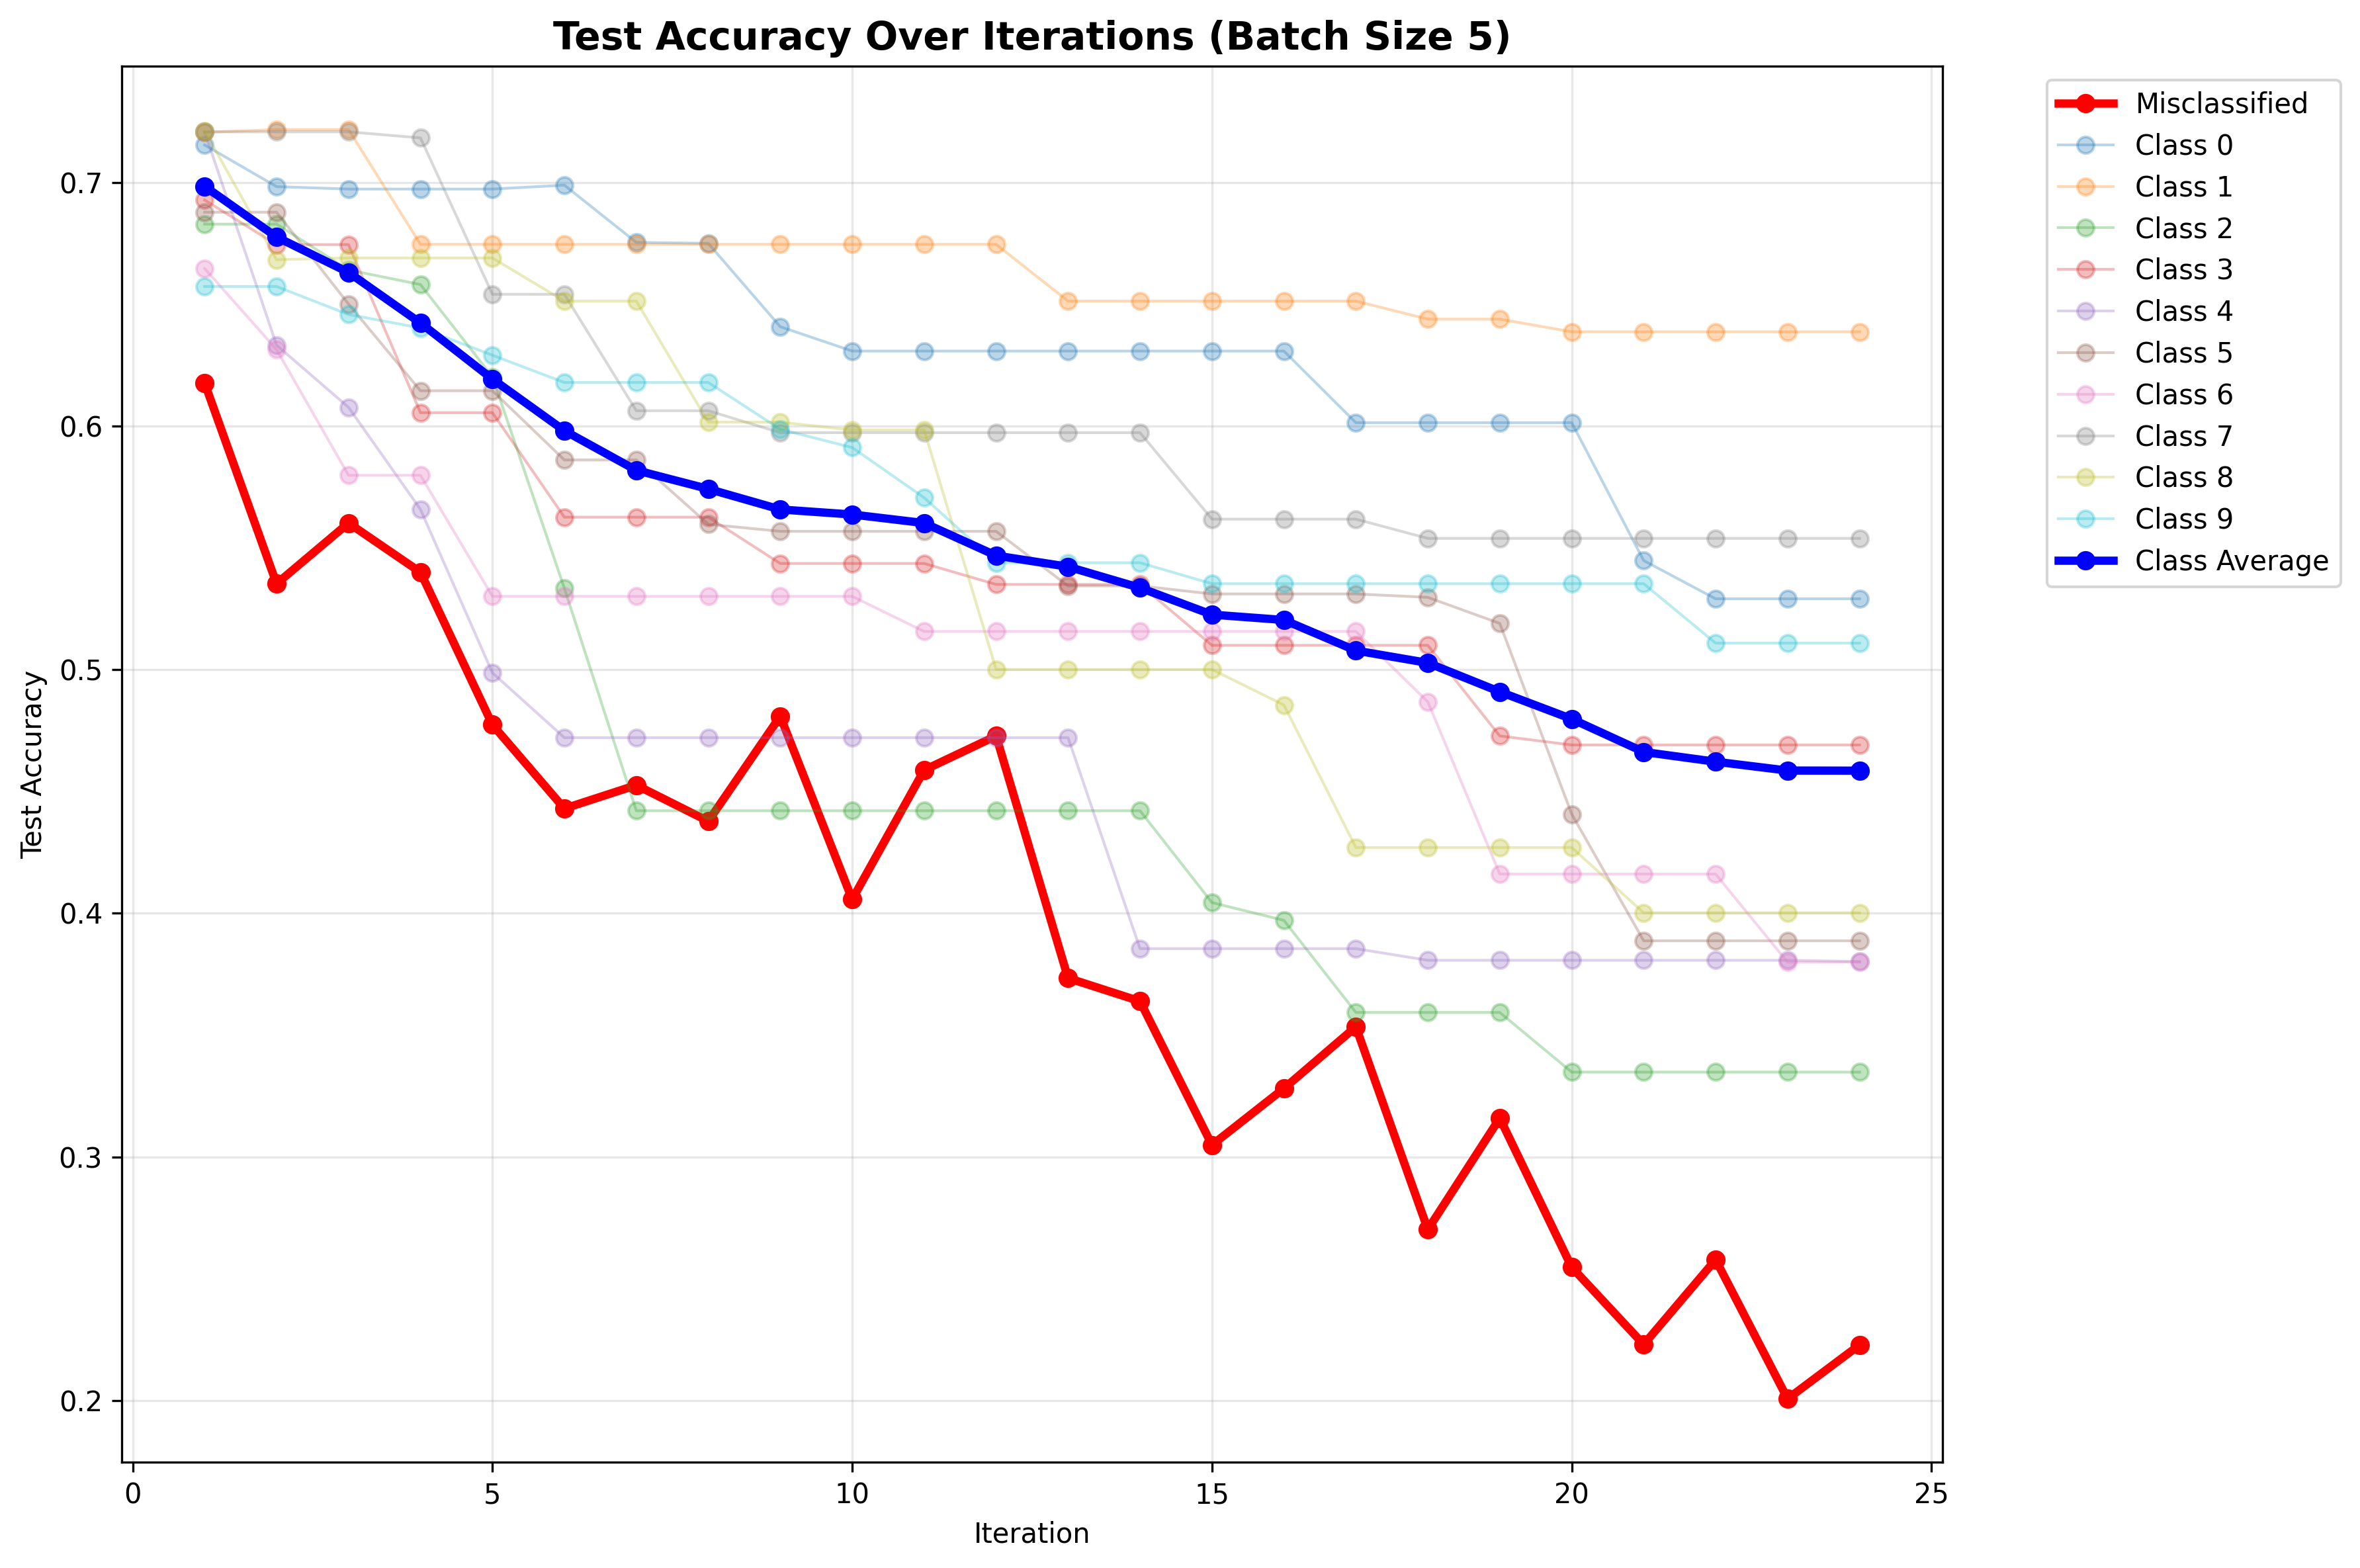
\includegraphics[width=\textwidth]{results/stochastic_analysis/batch_iterations/test_accuracy_batch_5.png}
	\caption{Test accuracy evolution for batch size 5 showing that early stopping around iteration 5 would preserve much higher global accuracy while maintaining excellent repair set performance.}
	\label{fig:early_stopping_batch_5}
\end{figure}

\begin{figure}[h]
	\centering
	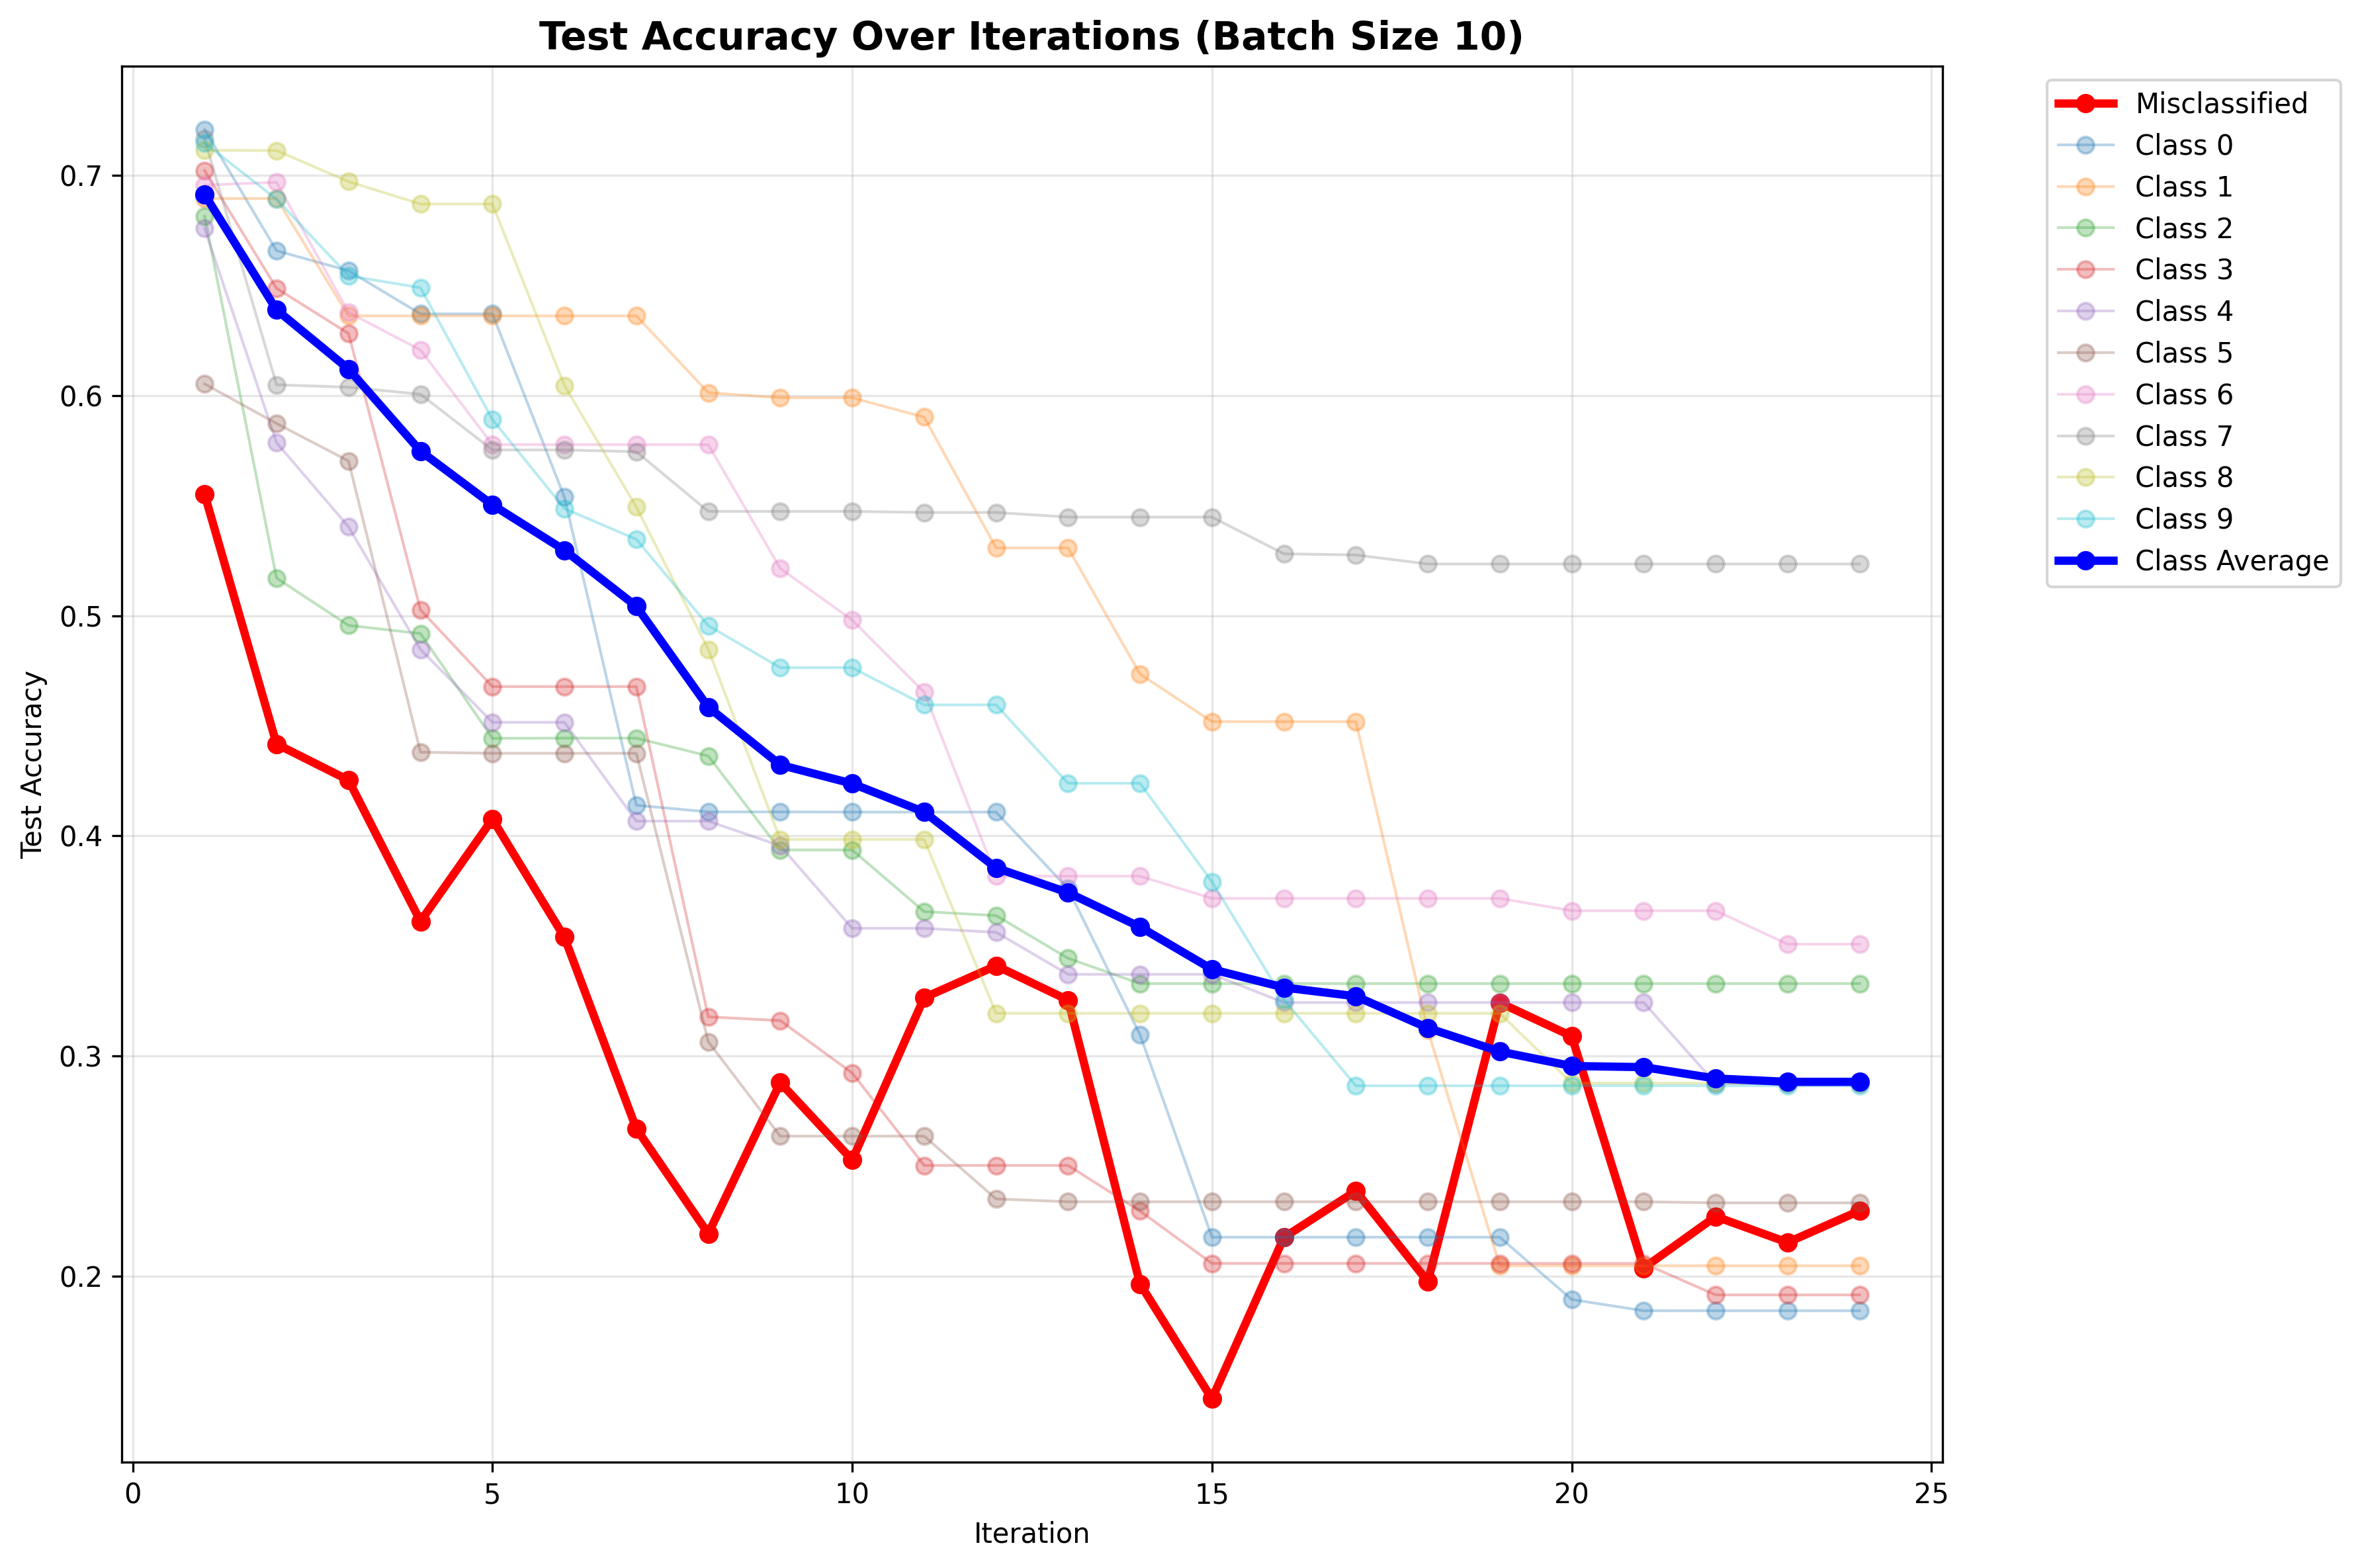
\includegraphics[width=\textwidth]{results/stochastic_analysis/batch_iterations/test_accuracy_batch_10.png}
	\caption{Test accuracy evolution for batch size 10 demonstrating similar early stopping opportunities to reduce drawdown.}
	\label{fig:early_stopping_batch_10}
\end{figure}

Key findings from our analysis show that:
\begin{itemize}
	\item \textbf{Rapid Convergence:} Class-homogeneous repairs reach 99\% repair set accuracy within 5 iterations
	\item \textbf{Early Stopping Benefit:} Stopping at iteration 5 preserves 60-65\% test accuracy vs. 45-29\% when running to completion
	\item \textbf{Batch Size Efficiency:} Both batch sizes 5 and 10 show similar convergence patterns, with batch 5 being slightly more stable
\end{itemize}

\subsection{Cross-Architecture Analysis and Implications}

Our comprehensive evaluation across both simple MLP models and complex CNN architectures reveals fundamental insights about heuristic effectiveness and the nature of neural network repair.

\subsubsection{Architecture-Dependent Heuristic Performance}

\textbf{Model Complexity and Repair Sensitivity:} Our MLP experiments demonstrate that simpler models with clear geometric decision boundaries respond well to targeted parameter modifications. The WeightsActivationBased heuristic's success (achieving +3.66\% improvement) illustrates how activation-guided weight adjustments can effectively reshape decision boundaries without catastrophic interference. This mirrors the intuitive process of adjusting polynomial coefficients to better fit data points—small, targeted changes to critical parameters can yield significant improvements in model behavior.

\textbf{Scaling Challenges in Complex Models:} In contrast, our CNN experiments on CIFAR-10 reveal the increased difficulty of repair in high-dimensional parameter spaces. The dramatic performance degradation observed in AlexNet repairs (up to -50.8% accuracy drawdown for large repair sets) suggests that complex models are more susceptible to parameter interference effects. This aligns with the understanding that CNNs learn hierarchical feature representations where modifications to early layers can cascade through the entire network.

\textbf{Set Heuristic Effectiveness Patterns:} The ConfidenceBased set heuristic's superior performance in MLP experiments (+3.66\% with WeightsActivationBased) demonstrates the value of principled sample selection. Low-confidence predictions often correspond to points near decision boundaries, making them ideal targets for local repairs that preserve global model behavior.

\subsubsection{Fundamental Trade-offs in Neural Network Repair}

Our experiments reveal several critical trade-offs that practitioners must navigate:

\begin{enumerate}
	\item \textbf{Model Complexity vs. Repair Feasibility:} Simpler models (MLPs) show higher repair success rates and more predictable outcomes, while complex models (CNNs) exhibit greater sensitivity to parameter modifications and higher failure rates.

	\item \textbf{Repair Set Size vs. Global Performance:} Both architectures demonstrate that larger repair sets lead to worse global performance, but the degradation is more severe in complex models. CNN experiments show success rates dropping from 100\% (size 10) to 9.1\% (size 200), while MLP repairs maintain higher success rates across different set sizes.

	\item \textbf{Local Accuracy vs. Generalization:} The rapid convergence observed in CNN stochastic repair (99\% repair set accuracy within 5 iterations) comes at the cost of significant global accuracy degradation, highlighting the fundamental tension between local correctness and generalization.

	\item \textbf{Heuristic Sophistication vs. Robustness:} Advanced heuristics (Adversarial, GradientBased) showed higher failure rates in our MLP experiments, suggesting that simpler, more robust approaches may be preferable for practical deployment.
\end{enumerate}

\subsubsection{Implications for Repair Strategy Selection}
\begin{itemize}
	\item Repair set curation is critical—semantic coherence significantly improves outcomes
	\item Size limitations exist for all architectures, though thresholds vary
	\item Confidence-based sample selection outperforms naive misclassification targeting
	\item One-shot repairs generally preserve global performance better than iterative approaches
\end{itemize}

\subsubsection{Practical Implications}

These findings have important implications for practical DNN repair deployment:

\begin{itemize}
	\item \textbf{Repair Set Curation}: Careful selection and grouping of repair examples by semantic similarity can substantially improve repair outcomes.
	\item \textbf{Size Limitations}: There exist practical upper bounds on repair set size beyond which the cure becomes worse than the disease.
	\item \textbf{Strategy Selection}: One-shot repair is generally preferable to iterative approaches for maintaining global model performance.
	\item \textbf{Monitoring Requirements}: Any repair strategy requires careful post-repair validation to ensure acceptable global performance retention.
\end{itemize}

This geometric intuition suggests that repair effectiveness is fundamentally linked to the interpretability and locality of a model's decision-making process.

\section{Conclusions and Future Work}

Our comprehensive evaluation of informed neural network repair strategies across multiple architectures reveals fundamental insights about the nature of neural network modification and the effectiveness of principled heuristic guidance. Through systematic evaluation of 90 heuristic combinations on MLPs and extensive analysis of repair strategies on CNNs, we have established both the promise and limitations of guided repair approaches.

\textbf{Key Contributions and Findings:}

Our experimental results demonstrate that intelligent heuristic selection can significantly improve repair outcomes. The WeightsActivationBased + ConfidenceBased combination achieved a remarkable +3.66\% improvement over baseline MLP performance, showcasing the potential for substantial model enhancement through principled parameter modification. This success illustrates a key insight: for models with interpretable decision boundaries, targeted parameter adjustments function analogously to coefficient optimization in polynomial fitting, enabling precise control over model behavior.

The effectiveness of confidence-based set selection across both architectures validates our hypothesis that principled sample curation outperforms naive approaches. By targeting low-confidence predictions—often corresponding to decision boundary regions—we can achieve more effective repairs with less risk of global performance degradation.

Our cross-architectural analysis reveals a fundamental scaling challenge: repair complexity and failure rates increase dramatically with model sophistication. While simple MLPs demonstrate robust improvements with appropriate heuristics, complex CNNs exhibit severe sensitivity to repair interventions, with accuracy drawdowns reaching -50.8\% for large repair sets. This scaling behavior suggests that repair strategies must be carefully tailored to model complexity.

\textbf{Future Research Directions:}

Our work opens several promising avenues for future investigation:

\begin{itemize}
	\item Regularization techniques that preserve global decision boundaries while enabling local corrections
	\item Sophisticated layer selection heuristics that minimize repair impact on unrelated model functionality
	\item Adaptive repair strategies that adjust their approach based on repair set characteristics
	\item Multi-objective optimization frameworks that balance local repair success against global performance preservation
\end{itemize}

\textbf{Broader Impact:}

This work contributes to the broader goal of trustworthy AI by making neural network repair more systematic and predictable. By providing principled guidance for repair strategy selection, we help move the field away from ad-hoc approaches toward evidence-based practices. The geometric insights we provide also contribute to our theoretical understanding of neural network parameter spaces and their modification.

Ultimately, our findings demonstrate that while neural network repair remains a challenging problem, informed heuristic selection can significantly improve outcomes. The path forward requires continued research into architecture-specific strategies, better theoretical understanding of parameter modification effects, and the development of more sophisticated tools for predicting and controlling repair outcomes. Through such advances, we can work toward making neural network repair a reliable tool for enhancing AI system trustworthiness and safety.

\section{GitHub}

The code used in this project are available in the following two repos:
\begin{itemize}
	\item \textbf{For MLP experiments:} \url{https://github.com/Iemontine/informed-repair-dnns}
	\item \textbf{For AlexNet experiments:} \url{https://github.com/AkshatAdsule/alexnet_repair}
\end{itemize}

\newpage
\bibliographystyle{unsrt}
\bibliography{references}

\end{document}